
% Default to the notebook output style




% Inherit from the specified cell style.





\documentclass[11pt]{article}



    \usepackage[T1]{fontenc}
    % Nicer default font (+ math font) than Computer Modern for most use cases
    \usepackage{mathpazo}

    % Basic figure setup, for now with no caption control since it's done
    % automatically by Pandoc (which extracts ![](path) syntax from Markdown).
    \usepackage{graphicx}
    % We will generate all images so they have a width \maxwidth. This means
    % that they will get their normal width if they fit onto the page, but
    % are scaled down if they would overflow the margins.
    \makeatletter
    \def\maxwidth{\ifdim\Gin@nat@width>\linewidth\linewidth
    \else\Gin@nat@width\fi}
    \makeatother
    \let\Oldincludegraphics\includegraphics
    % Set max figure width to be 80% of text width, for now hardcoded.
    \renewcommand{\includegraphics}[1]{\Oldincludegraphics[width=.9\maxwidth]{#1}}
    % Ensure that by default, figures have no caption (until we provide a
    % proper Figure object with a Caption API and a way to capture that
    % in the conversion process - todo).
    \usepackage{caption}
    \DeclareCaptionLabelFormat{nolabel}{}
    \captionsetup{labelformat=nolabel}

    \usepackage{adjustbox} % Used to constrain images to a maximum size
    \usepackage{xcolor} % Allow colors to be defined
    \usepackage{enumerate} % Needed for markdown enumerations to work
    \usepackage{geometry} % Used to adjust the document margins
    \usepackage{amsmath} % Equations
    \usepackage{amssymb} % Equations
    \usepackage{textcomp} % defines textquotesingle
    % Hack from http://tex.stackexchange.com/a/47451/13684:
    \AtBeginDocument{%
        \def\PYZsq{\textquotesingle}% Upright quotes in Pygmentized code
    }
    \usepackage{upquote} % Upright quotes for verbatim code
    \usepackage{eurosym} % defines \euro
    \usepackage[mathletters]{ucs} % Extended unicode (utf-8) support
    \usepackage[utf8x]{inputenc} % Allow utf-8 characters in the tex document
    \usepackage{fancyvrb} % verbatim replacement that allows latex
    \usepackage{grffile} % extends the file name processing of package graphics
                         % to support a larger range
    % The hyperref package gives us a pdf with properly built
    % internal navigation ('pdf bookmarks' for the table of contents,
    % internal cross-reference links, web links for URLs, etc.)
    \usepackage{hyperref}
    \usepackage{longtable} % longtable support required by pandoc >1.10
    \usepackage{booktabs}  % table support for pandoc > 1.12.2
    \usepackage[inline]{enumitem} % IRkernel/repr support (it uses the enumerate* environment)
    \usepackage[normalem]{ulem} % ulem is needed to support strikethroughs (\sout)
                                % normalem makes italics be italics, not underlines
    \usepackage{mathrsfs}




    % Colors for the hyperref package
    \definecolor{urlcolor}{rgb}{0,.145,.698}
    \definecolor{linkcolor}{rgb}{.71,0.21,0.01}
    \definecolor{citecolor}{rgb}{.12,.54,.11}

    % ANSI colors
    \definecolor{ansi-black}{HTML}{3E424D}
    \definecolor{ansi-black-intense}{HTML}{282C36}
    \definecolor{ansi-red}{HTML}{E75C58}
    \definecolor{ansi-red-intense}{HTML}{B22B31}
    \definecolor{ansi-green}{HTML}{00A250}
    \definecolor{ansi-green-intense}{HTML}{007427}
    \definecolor{ansi-yellow}{HTML}{DDB62B}
    \definecolor{ansi-yellow-intense}{HTML}{B27D12}
    \definecolor{ansi-blue}{HTML}{208FFB}
    \definecolor{ansi-blue-intense}{HTML}{0065CA}
    \definecolor{ansi-magenta}{HTML}{D160C4}
    \definecolor{ansi-magenta-intense}{HTML}{A03196}
    \definecolor{ansi-cyan}{HTML}{60C6C8}
    \definecolor{ansi-cyan-intense}{HTML}{258F8F}
    \definecolor{ansi-white}{HTML}{C5C1B4}
    \definecolor{ansi-white-intense}{HTML}{A1A6B2}
    \definecolor{ansi-default-inverse-fg}{HTML}{FFFFFF}
    \definecolor{ansi-default-inverse-bg}{HTML}{000000}

    % commands and environments needed by pandoc snippets
    % extracted from the output of `pandoc -s`
    \providecommand{\tightlist}{%
      \setlength{\itemsep}{0pt}\setlength{\parskip}{0pt}}
    \DefineVerbatimEnvironment{Highlighting}{Verbatim}{commandchars=\\\{\}}
    % Add ',fontsize=\small' for more characters per line
    \newenvironment{Shaded}{}{}
    \newcommand{\KeywordTok}[1]{\textcolor[rgb]{0.00,0.44,0.13}{\textbf{{#1}}}}
    \newcommand{\DataTypeTok}[1]{\textcolor[rgb]{0.56,0.13,0.00}{{#1}}}
    \newcommand{\DecValTok}[1]{\textcolor[rgb]{0.25,0.63,0.44}{{#1}}}
    \newcommand{\BaseNTok}[1]{\textcolor[rgb]{0.25,0.63,0.44}{{#1}}}
    \newcommand{\FloatTok}[1]{\textcolor[rgb]{0.25,0.63,0.44}{{#1}}}
    \newcommand{\CharTok}[1]{\textcolor[rgb]{0.25,0.44,0.63}{{#1}}}
    \newcommand{\StringTok}[1]{\textcolor[rgb]{0.25,0.44,0.63}{{#1}}}
    \newcommand{\CommentTok}[1]{\textcolor[rgb]{0.38,0.63,0.69}{\textit{{#1}}}}
    \newcommand{\OtherTok}[1]{\textcolor[rgb]{0.00,0.44,0.13}{{#1}}}
    \newcommand{\AlertTok}[1]{\textcolor[rgb]{1.00,0.00,0.00}{\textbf{{#1}}}}
    \newcommand{\FunctionTok}[1]{\textcolor[rgb]{0.02,0.16,0.49}{{#1}}}
    \newcommand{\RegionMarkerTok}[1]{{#1}}
    \newcommand{\ErrorTok}[1]{\textcolor[rgb]{1.00,0.00,0.00}{\textbf{{#1}}}}
    \newcommand{\NormalTok}[1]{{#1}}

    % Additional commands for more recent versions of Pandoc
    \newcommand{\ConstantTok}[1]{\textcolor[rgb]{0.53,0.00,0.00}{{#1}}}
    \newcommand{\SpecialCharTok}[1]{\textcolor[rgb]{0.25,0.44,0.63}{{#1}}}
    \newcommand{\VerbatimStringTok}[1]{\textcolor[rgb]{0.25,0.44,0.63}{{#1}}}
    \newcommand{\SpecialStringTok}[1]{\textcolor[rgb]{0.73,0.40,0.53}{{#1}}}
    \newcommand{\ImportTok}[1]{{#1}}
    \newcommand{\DocumentationTok}[1]{\textcolor[rgb]{0.73,0.13,0.13}{\textit{{#1}}}}
    \newcommand{\AnnotationTok}[1]{\textcolor[rgb]{0.38,0.63,0.69}{\textbf{\textit{{#1}}}}}
    \newcommand{\CommentVarTok}[1]{\textcolor[rgb]{0.38,0.63,0.69}{\textbf{\textit{{#1}}}}}
    \newcommand{\VariableTok}[1]{\textcolor[rgb]{0.10,0.09,0.49}{{#1}}}
    \newcommand{\ControlFlowTok}[1]{\textcolor[rgb]{0.00,0.44,0.13}{\textbf{{#1}}}}
    \newcommand{\OperatorTok}[1]{\textcolor[rgb]{0.40,0.40,0.40}{{#1}}}
    \newcommand{\BuiltInTok}[1]{{#1}}
    \newcommand{\ExtensionTok}[1]{{#1}}
    \newcommand{\PreprocessorTok}[1]{\textcolor[rgb]{0.74,0.48,0.00}{{#1}}}
    \newcommand{\AttributeTok}[1]{\textcolor[rgb]{0.49,0.56,0.16}{{#1}}}
    \newcommand{\InformationTok}[1]{\textcolor[rgb]{0.38,0.63,0.69}{\textbf{\textit{{#1}}}}}
    \newcommand{\WarningTok}[1]{\textcolor[rgb]{0.38,0.63,0.69}{\textbf{\textit{{#1}}}}}


    % Define a nice break command that doesn't care if a line doesn't already
    % exist.
    \def\br{\hspace*{\fill} \\* }
    % Math Jax compatibility definitions
    \def\gt{>}
    \def\lt{<}
    \let\Oldtex\TeX
    \let\Oldlatex\LaTeX
    \renewcommand{\TeX}{\textrm{\Oldtex}}
    \renewcommand{\LaTeX}{\textrm{\Oldlatex}}
    % Document parameters
    % Document title
    \title{Código }






    % Pygments definitions

\makeatletter
\def\PY@reset{\let\PY@it=\relax \let\PY@bf=\relax%
    \let\PY@ul=\relax \let\PY@tc=\relax%
    \let\PY@bc=\relax \let\PY@ff=\relax}
\def\PY@tok#1{\csname PY@tok@#1\endcsname}
\def\PY@toks#1+{\ifx\relax#1\empty\else%
    \PY@tok{#1}\expandafter\PY@toks\fi}
\def\PY@do#1{\PY@bc{\PY@tc{\PY@ul{%
    \PY@it{\PY@bf{\PY@ff{#1}}}}}}}
\def\PY#1#2{\PY@reset\PY@toks#1+\relax+\PY@do{#2}}

\expandafter\def\csname PY@tok@w\endcsname{\def\PY@tc##1{\textcolor[rgb]{0.73,0.73,0.73}{##1}}}
\expandafter\def\csname PY@tok@c\endcsname{\let\PY@it=\textit\def\PY@tc##1{\textcolor[rgb]{0.25,0.50,0.50}{##1}}}
\expandafter\def\csname PY@tok@cp\endcsname{\def\PY@tc##1{\textcolor[rgb]{0.74,0.48,0.00}{##1}}}
\expandafter\def\csname PY@tok@k\endcsname{\let\PY@bf=\textbf\def\PY@tc##1{\textcolor[rgb]{0.00,0.50,0.00}{##1}}}
\expandafter\def\csname PY@tok@kp\endcsname{\def\PY@tc##1{\textcolor[rgb]{0.00,0.50,0.00}{##1}}}
\expandafter\def\csname PY@tok@kt\endcsname{\def\PY@tc##1{\textcolor[rgb]{0.69,0.00,0.25}{##1}}}
\expandafter\def\csname PY@tok@o\endcsname{\def\PY@tc##1{\textcolor[rgb]{0.40,0.40,0.40}{##1}}}
\expandafter\def\csname PY@tok@ow\endcsname{\let\PY@bf=\textbf\def\PY@tc##1{\textcolor[rgb]{0.67,0.13,1.00}{##1}}}
\expandafter\def\csname PY@tok@nb\endcsname{\def\PY@tc##1{\textcolor[rgb]{0.00,0.50,0.00}{##1}}}
\expandafter\def\csname PY@tok@nf\endcsname{\def\PY@tc##1{\textcolor[rgb]{0.00,0.00,1.00}{##1}}}
\expandafter\def\csname PY@tok@nc\endcsname{\let\PY@bf=\textbf\def\PY@tc##1{\textcolor[rgb]{0.00,0.00,1.00}{##1}}}
\expandafter\def\csname PY@tok@nn\endcsname{\let\PY@bf=\textbf\def\PY@tc##1{\textcolor[rgb]{0.00,0.00,1.00}{##1}}}
\expandafter\def\csname PY@tok@ne\endcsname{\let\PY@bf=\textbf\def\PY@tc##1{\textcolor[rgb]{0.82,0.25,0.23}{##1}}}
\expandafter\def\csname PY@tok@nv\endcsname{\def\PY@tc##1{\textcolor[rgb]{0.10,0.09,0.49}{##1}}}
\expandafter\def\csname PY@tok@no\endcsname{\def\PY@tc##1{\textcolor[rgb]{0.53,0.00,0.00}{##1}}}
\expandafter\def\csname PY@tok@nl\endcsname{\def\PY@tc##1{\textcolor[rgb]{0.63,0.63,0.00}{##1}}}
\expandafter\def\csname PY@tok@ni\endcsname{\let\PY@bf=\textbf\def\PY@tc##1{\textcolor[rgb]{0.60,0.60,0.60}{##1}}}
\expandafter\def\csname PY@tok@na\endcsname{\def\PY@tc##1{\textcolor[rgb]{0.49,0.56,0.16}{##1}}}
\expandafter\def\csname PY@tok@nt\endcsname{\let\PY@bf=\textbf\def\PY@tc##1{\textcolor[rgb]{0.00,0.50,0.00}{##1}}}
\expandafter\def\csname PY@tok@nd\endcsname{\def\PY@tc##1{\textcolor[rgb]{0.67,0.13,1.00}{##1}}}
\expandafter\def\csname PY@tok@s\endcsname{\def\PY@tc##1{\textcolor[rgb]{0.73,0.13,0.13}{##1}}}
\expandafter\def\csname PY@tok@sd\endcsname{\let\PY@it=\textit\def\PY@tc##1{\textcolor[rgb]{0.73,0.13,0.13}{##1}}}
\expandafter\def\csname PY@tok@si\endcsname{\let\PY@bf=\textbf\def\PY@tc##1{\textcolor[rgb]{0.73,0.40,0.53}{##1}}}
\expandafter\def\csname PY@tok@se\endcsname{\let\PY@bf=\textbf\def\PY@tc##1{\textcolor[rgb]{0.73,0.40,0.13}{##1}}}
\expandafter\def\csname PY@tok@sr\endcsname{\def\PY@tc##1{\textcolor[rgb]{0.73,0.40,0.53}{##1}}}
\expandafter\def\csname PY@tok@ss\endcsname{\def\PY@tc##1{\textcolor[rgb]{0.10,0.09,0.49}{##1}}}
\expandafter\def\csname PY@tok@sx\endcsname{\def\PY@tc##1{\textcolor[rgb]{0.00,0.50,0.00}{##1}}}
\expandafter\def\csname PY@tok@m\endcsname{\def\PY@tc##1{\textcolor[rgb]{0.40,0.40,0.40}{##1}}}
\expandafter\def\csname PY@tok@gh\endcsname{\let\PY@bf=\textbf\def\PY@tc##1{\textcolor[rgb]{0.00,0.00,0.50}{##1}}}
\expandafter\def\csname PY@tok@gu\endcsname{\let\PY@bf=\textbf\def\PY@tc##1{\textcolor[rgb]{0.50,0.00,0.50}{##1}}}
\expandafter\def\csname PY@tok@gd\endcsname{\def\PY@tc##1{\textcolor[rgb]{0.63,0.00,0.00}{##1}}}
\expandafter\def\csname PY@tok@gi\endcsname{\def\PY@tc##1{\textcolor[rgb]{0.00,0.63,0.00}{##1}}}
\expandafter\def\csname PY@tok@gr\endcsname{\def\PY@tc##1{\textcolor[rgb]{1.00,0.00,0.00}{##1}}}
\expandafter\def\csname PY@tok@ge\endcsname{\let\PY@it=\textit}
\expandafter\def\csname PY@tok@gs\endcsname{\let\PY@bf=\textbf}
\expandafter\def\csname PY@tok@gp\endcsname{\let\PY@bf=\textbf\def\PY@tc##1{\textcolor[rgb]{0.00,0.00,0.50}{##1}}}
\expandafter\def\csname PY@tok@go\endcsname{\def\PY@tc##1{\textcolor[rgb]{0.53,0.53,0.53}{##1}}}
\expandafter\def\csname PY@tok@gt\endcsname{\def\PY@tc##1{\textcolor[rgb]{0.00,0.27,0.87}{##1}}}
\expandafter\def\csname PY@tok@err\endcsname{\def\PY@bc##1{\setlength{\fboxsep}{0pt}\fcolorbox[rgb]{1.00,0.00,0.00}{1,1,1}{\strut ##1}}}
\expandafter\def\csname PY@tok@kc\endcsname{\let\PY@bf=\textbf\def\PY@tc##1{\textcolor[rgb]{0.00,0.50,0.00}{##1}}}
\expandafter\def\csname PY@tok@kd\endcsname{\let\PY@bf=\textbf\def\PY@tc##1{\textcolor[rgb]{0.00,0.50,0.00}{##1}}}
\expandafter\def\csname PY@tok@kn\endcsname{\let\PY@bf=\textbf\def\PY@tc##1{\textcolor[rgb]{0.00,0.50,0.00}{##1}}}
\expandafter\def\csname PY@tok@kr\endcsname{\let\PY@bf=\textbf\def\PY@tc##1{\textcolor[rgb]{0.00,0.50,0.00}{##1}}}
\expandafter\def\csname PY@tok@bp\endcsname{\def\PY@tc##1{\textcolor[rgb]{0.00,0.50,0.00}{##1}}}
\expandafter\def\csname PY@tok@fm\endcsname{\def\PY@tc##1{\textcolor[rgb]{0.00,0.00,1.00}{##1}}}
\expandafter\def\csname PY@tok@vc\endcsname{\def\PY@tc##1{\textcolor[rgb]{0.10,0.09,0.49}{##1}}}
\expandafter\def\csname PY@tok@vg\endcsname{\def\PY@tc##1{\textcolor[rgb]{0.10,0.09,0.49}{##1}}}
\expandafter\def\csname PY@tok@vi\endcsname{\def\PY@tc##1{\textcolor[rgb]{0.10,0.09,0.49}{##1}}}
\expandafter\def\csname PY@tok@vm\endcsname{\def\PY@tc##1{\textcolor[rgb]{0.10,0.09,0.49}{##1}}}
\expandafter\def\csname PY@tok@sa\endcsname{\def\PY@tc##1{\textcolor[rgb]{0.73,0.13,0.13}{##1}}}
\expandafter\def\csname PY@tok@sb\endcsname{\def\PY@tc##1{\textcolor[rgb]{0.73,0.13,0.13}{##1}}}
\expandafter\def\csname PY@tok@sc\endcsname{\def\PY@tc##1{\textcolor[rgb]{0.73,0.13,0.13}{##1}}}
\expandafter\def\csname PY@tok@dl\endcsname{\def\PY@tc##1{\textcolor[rgb]{0.73,0.13,0.13}{##1}}}
\expandafter\def\csname PY@tok@s2\endcsname{\def\PY@tc##1{\textcolor[rgb]{0.73,0.13,0.13}{##1}}}
\expandafter\def\csname PY@tok@sh\endcsname{\def\PY@tc##1{\textcolor[rgb]{0.73,0.13,0.13}{##1}}}
\expandafter\def\csname PY@tok@s1\endcsname{\def\PY@tc##1{\textcolor[rgb]{0.73,0.13,0.13}{##1}}}
\expandafter\def\csname PY@tok@mb\endcsname{\def\PY@tc##1{\textcolor[rgb]{0.40,0.40,0.40}{##1}}}
\expandafter\def\csname PY@tok@mf\endcsname{\def\PY@tc##1{\textcolor[rgb]{0.40,0.40,0.40}{##1}}}
\expandafter\def\csname PY@tok@mh\endcsname{\def\PY@tc##1{\textcolor[rgb]{0.40,0.40,0.40}{##1}}}
\expandafter\def\csname PY@tok@mi\endcsname{\def\PY@tc##1{\textcolor[rgb]{0.40,0.40,0.40}{##1}}}
\expandafter\def\csname PY@tok@il\endcsname{\def\PY@tc##1{\textcolor[rgb]{0.40,0.40,0.40}{##1}}}
\expandafter\def\csname PY@tok@mo\endcsname{\def\PY@tc##1{\textcolor[rgb]{0.40,0.40,0.40}{##1}}}
\expandafter\def\csname PY@tok@ch\endcsname{\let\PY@it=\textit\def\PY@tc##1{\textcolor[rgb]{0.25,0.50,0.50}{##1}}}
\expandafter\def\csname PY@tok@cm\endcsname{\let\PY@it=\textit\def\PY@tc##1{\textcolor[rgb]{0.25,0.50,0.50}{##1}}}
\expandafter\def\csname PY@tok@cpf\endcsname{\let\PY@it=\textit\def\PY@tc##1{\textcolor[rgb]{0.25,0.50,0.50}{##1}}}
\expandafter\def\csname PY@tok@c1\endcsname{\let\PY@it=\textit\def\PY@tc##1{\textcolor[rgb]{0.25,0.50,0.50}{##1}}}
\expandafter\def\csname PY@tok@cs\endcsname{\let\PY@it=\textit\def\PY@tc##1{\textcolor[rgb]{0.25,0.50,0.50}{##1}}}

\def\PYZbs{\char`\\}
\def\PYZus{\char`\_}
\def\PYZob{\char`\{}
\def\PYZcb{\char`\}}
\def\PYZca{\char`\^}
\def\PYZam{\char`\&}
\def\PYZlt{\char`\<}
\def\PYZgt{\char`\>}
\def\PYZsh{\char`\#}
\def\PYZpc{\char`\%}
\def\PYZdl{\char`\$}
\def\PYZhy{\char`\-}
\def\PYZsq{\char`\'}
\def\PYZdq{\char`\"}
\def\PYZti{\char`\~}
% for compatibility with earlier versions
\def\PYZat{@}
\def\PYZlb{[}
\def\PYZrb{]}
\makeatother


    % Exact colors from NB
    \definecolor{incolor}{rgb}{0.0, 0.0, 0.5}
    \definecolor{outcolor}{rgb}{0.545, 0.0, 0.0}




    % Prevent overflowing lines due to hard-to-break entities
    \sloppy
    % Setup hyperref package
    \hypersetup{
      breaklinks=true,  % so long urls are correctly broken across lines
      colorlinks=true,
      urlcolor=urlcolor,
      linkcolor=linkcolor,
      citecolor=citecolor,
      }
    % Slightly bigger margins than the latex defaults

    \geometry{verbose,tmargin=1in,bmargin=1in,lmargin=1in,rmargin=1in}



    \begin{document}

\pagestyle{empty}





    \section{Sistema de clasificación de estilo de
manejo}\label{sistema-de-clasificaciuxf3n-de-estilo-de-manejo}

    \subsection{1. Importando módulos}\label{importando-muxf3dulos}

    \begin{Verbatim}[commandchars=\\\{\}]
{\color{incolor}In [{\color{incolor}1}]:} \PY{k+kn}{import} \PY{n+nn}{os}
        \PY{k+kn}{import} \PY{n+nn}{pandas} \PY{k}{as} \PY{n+nn}{pd}
        \PY{k+kn}{import} \PY{n+nn}{numpy} \PY{k}{as} \PY{n+nn}{np}
        \PY{k+kn}{import} \PY{n+nn}{warnings}
        \PY{k+kn}{import} \PY{n+nn}{matplotlib}\PY{n+nn}{.}\PY{n+nn}{pyplot} \PY{k}{as} \PY{n+nn}{plt}
        \PY{k+kn}{import} \PY{n+nn}{matplotlib}\PY{n+nn}{.}\PY{n+nn}{gridspec} \PY{k}{as} \PY{n+nn}{gridspec}
        \PY{k+kn}{import} \PY{n+nn}{seaborn} \PY{k}{as} \PY{n+nn}{sns}
        \PY{n}{sns}\PY{o}{.}\PY{n}{set}\PY{p}{(}\PY{p}{)}
        \PY{k+kn}{from} \PY{n+nn}{statsmodels}\PY{n+nn}{.}\PY{n+nn}{graphics}\PY{n+nn}{.}\PY{n+nn}{mosaicplot} \PY{k}{import} \PY{n}{mosaic}
        \PY{k+kn}{import} \PY{n+nn}{math}
        \PY{k+kn}{from} \PY{n+nn}{sklearn}\PY{n+nn}{.}\PY{n+nn}{manifold} \PY{k}{import} \PY{n}{LocallyLinearEmbedding}
        \PY{k+kn}{from} \PY{n+nn}{mpl\PYZus{}toolkits}\PY{n+nn}{.}\PY{n+nn}{mplot3d} \PY{k}{import} \PY{n}{Axes3D}
\end{Verbatim}

    \subsection{2. Definir funciones}\label{definir-funciones}

    Se define una función para leer los 38 archivos 'csv' y otra para
dividir a los archivos en ventanas de tamaño w

\newpage

    \begin{Verbatim}[commandchars=\\\{\}]
{\color{incolor}In [{\color{incolor}2}]:} \PY{k}{def} \PY{n+nf}{car\PYZus{}trip\PYZus{}filename}\PY{p}{(}\PY{n}{n}\PY{p}{)}\PY{p}{:}
            \PY{k}{if} \PY{p}{(}\PY{n}{n}\PY{o}{\PYZlt{}}\PY{l+m+mi}{1}\PY{p}{)} \PY{o}{|} \PY{p}{(}\PY{n}{n}\PY{o}{\PYZgt{}}\PY{l+m+mi}{38}\PY{p}{)}\PY{p}{:}
                \PY{n+nb}{print}\PY{p}{(}\PY{l+s+s1}{\PYZsq{}}\PY{l+s+s1}{n out of the scope}\PY{l+s+s1}{\PYZsq{}}\PY{p}{)}
                \PY{k}{return} \PY{n}{np}\PY{o}{.}\PY{n}{NAN}
            \PY{n}{route\PYZus{}data\PYZus{}kaggle}\PY{o}{=}\PY{l+s+s1}{\PYZsq{}}\PY{l+s+s1}{../Datos/Car trips data log/TripData/Processed Data}\PY{l+s+s1}{\PYZsq{}}
            \PY{n}{processed\PYZus{}file\PYZus{}name}\PY{o}{=}\PY{l+s+s1}{\PYZsq{}}\PY{l+s+s1}{fileID}\PY{l+s+s1}{\PYZsq{}}\PY{o}{+}\PY{n+nb}{str}\PY{p}{(}\PY{n}{n}\PY{p}{)}\PY{o}{+}\PY{l+s+s1}{\PYZsq{}}\PY{l+s+s1}{\PYZus{}ProcessedTripData.csv}\PY{l+s+s1}{\PYZsq{}}
            \PY{n}{data} \PY{o}{=} \PY{n}{pd}\PY{o}{.}\PY{n}{read\PYZus{}csv}\PY{p}{(}\PY{n}{route\PYZus{}data\PYZus{}kaggle} \PY{o}{+} \PY{l+s+s1}{\PYZsq{}}\PY{l+s+s1}{/}\PY{l+s+s1}{\PYZsq{}} \PY{o}{+} \PY{n}{processed\PYZus{}file\PYZus{}name}\PY{p}{,} \PY{n}{delimiter} \PY{o}{=} \PY{l+s+s1}{\PYZsq{}}\PY{l+s+s1}{,}\PY{l+s+s1}{\PYZsq{}}\PY{p}{,}
                               \PY{n}{header}\PY{o}{=}\PY{k+kc}{None}\PY{p}{,}
                               \PY{n}{names}\PY{o}{=}\PY{p}{[}\PY{l+s+s1}{\PYZsq{}}\PY{l+s+s1}{Time(s)}\PY{l+s+s1}{\PYZsq{}}\PY{p}{,}
                                        \PY{l+s+s1}{\PYZsq{}}\PY{l+s+s1}{Speed(m/s)}\PY{l+s+s1}{\PYZsq{}}\PY{p}{,}
                                        \PY{l+s+s1}{\PYZsq{}}\PY{l+s+s1}{Shift\PYZus{}number}\PY{l+s+s1}{\PYZsq{}}\PY{p}{,}
                                        \PY{l+s+s1}{\PYZsq{}}\PY{l+s+s1}{Engine\PYZus{}Load(}\PY{l+s+s1}{\PYZpc{}}\PY{l+s+s1}{)}\PY{l+s+s1}{\PYZsq{}}\PY{p}{,}
                                        \PY{l+s+s1}{\PYZsq{}}\PY{l+s+s1}{Total\PYZus{}Acceleration(m/s\PYZca{}2)}\PY{l+s+s1}{\PYZsq{}}\PY{p}{,}
                                        \PY{l+s+s1}{\PYZsq{}}\PY{l+s+s1}{Engine RPM}\PY{l+s+s1}{\PYZsq{}}\PY{p}{,}
                                        \PY{l+s+s1}{\PYZsq{}}\PY{l+s+s1}{Pitch}\PY{l+s+s1}{\PYZsq{}}\PY{p}{,}
                                        \PY{l+s+s1}{\PYZsq{}}\PY{l+s+s1}{Lateral\PYZus{}Acceleration(m/s\PYZca{}2)}\PY{l+s+s1}{\PYZsq{}}\PY{p}{,}
                                        \PY{l+s+s1}{\PYZsq{}}\PY{l+s+s1}{Passenger\PYZus{}count(0\PYZhy{}5)}\PY{l+s+s1}{\PYZsq{}}\PY{p}{,}
                                        \PY{l+s+s1}{\PYZsq{}}\PY{l+s+s1}{Load(0\PYZhy{}10)}\PY{l+s+s1}{\PYZsq{}}\PY{p}{,}
                                        \PY{l+s+s1}{\PYZsq{}}\PY{l+s+s1}{Air\PYZus{}conditioning(0\PYZhy{}4)}\PY{l+s+s1}{\PYZsq{}}\PY{p}{,}
                                        \PY{l+s+s1}{\PYZsq{}}\PY{l+s+s1}{Window\PYZus{}opening(0\PYZhy{}10)}\PY{l+s+s1}{\PYZsq{}}\PY{p}{,}
                                        \PY{l+s+s1}{\PYZsq{}}\PY{l+s+s1}{Radio\PYZus{}volume(0\PYZhy{}10)}\PY{l+s+s1}{\PYZsq{}}\PY{p}{,}
                                        \PY{l+s+s1}{\PYZsq{}}\PY{l+s+s1}{Rain\PYZus{}intensity(0\PYZhy{}10)}\PY{l+s+s1}{\PYZsq{}}\PY{p}{,}
                                        \PY{l+s+s1}{\PYZsq{}}\PY{l+s+s1}{Visibility}\PY{l+s+s1}{\PYZsq{}}\PY{p}{,}
                                        \PY{l+s+s1}{\PYZsq{}}\PY{l+s+s1}{Driver\PYZus{}wellbeing(0\PYZhy{}10)}\PY{l+s+s1}{\PYZsq{}}\PY{p}{,}
                                        \PY{l+s+s1}{\PYZsq{}}\PY{l+s+s1}{Driver\PYZus{}rush(0\PYZhy{}10)}\PY{l+s+s1}{\PYZsq{}}\PY{p}{]}\PY{p}{)}
            \PY{k}{return} \PY{n}{data}

        \PY{k}{def} \PY{n+nf}{read\PYZus{}all}\PY{p}{(}\PY{p}{)}\PY{p}{:}
            \PY{n}{Data}\PY{o}{=}\PY{p}{[}\PY{p}{]}
            \PY{k}{for} \PY{n}{n\PYZus{}file} \PY{o+ow}{in} \PY{n+nb}{range}\PY{p}{(}\PY{l+m+mi}{1}\PY{p}{,}\PY{l+m+mi}{39}\PY{p}{)}\PY{p}{:}
                \PY{n}{Data}\PY{o}{.}\PY{n}{append}\PY{p}{(}\PY{n}{car\PYZus{}trip\PYZus{}filename}\PY{p}{(}\PY{n}{n\PYZus{}file}\PY{p}{)}\PY{p}{)}
            \PY{k}{return} \PY{n}{Data}

        \PY{c+c1}{\PYZsh{}Obtiene una lista con los valores de duración en segundos de cada }
        \PY{k}{def} \PY{n+nf}{duracion\PYZus{}total\PYZus{}sec}\PY{p}{(}\PY{n}{Data}\PY{p}{)}\PY{p}{:}
            \PY{n}{duration\PYZus{}sec}\PY{o}{=}\PY{p}{[}\PY{p}{]}
            \PY{k}{for} \PY{n}{m} \PY{o+ow}{in} \PY{n+nb}{range}\PY{p}{(}\PY{n+nb}{len}\PY{p}{(}\PY{n}{Data}\PY{p}{)}\PY{p}{)}\PY{p}{:}
                \PY{n}{duration\PYZus{}sec}\PY{o}{.}\PY{n}{append}\PY{p}{(}\PY{n}{Data}\PY{p}{[}\PY{n}{m}\PY{p}{]}\PY{o}{.}\PY{n}{iloc}\PY{p}{[}\PY{n}{Data}\PY{p}{[}\PY{n}{m}\PY{p}{]}\PY{o}{.}\PY{n}{shape}\PY{p}{[}\PY{l+m+mi}{0}\PY{p}{]}\PY{o}{\PYZhy{}}\PY{l+m+mi}{1}\PY{p}{,}\PY{l+m+mi}{0}\PY{p}{]}\PY{o}{\PYZhy{}}\PY{n}{Data}\PY{p}{[}\PY{n}{m}\PY{p}{]}\PY{o}{.}\PY{n}{iloc}\PY{p}{[}\PY{l+m+mi}{0}\PY{p}{,}\PY{l+m+mi}{0}\PY{p}{]}\PY{p}{)}
            \PY{k}{return} \PY{n}{duration\PYZus{}sec}

        \PY{c+c1}{\PYZsh{} Obtiene un diccionario en el que las \PYZsq{}keys\PYZsq{} son los indices de Data }
        \PY{c+c1}{\PYZsh{}(representando el número de archivo) y }
        \PY{c+c1}{\PYZsh{} el \PYZsq{}value\PYZsq{} es una lista con la duración entre cada fila en segundos}
        \PY{k}{def} \PY{n+nf}{dict\PYZus{}with\PYZus{}step}\PY{p}{(}\PY{n}{Data}\PY{p}{)}\PY{p}{:}
            \PY{n}{dict\PYZus{}period}\PY{o}{=}\PY{p}{\PYZob{}}\PY{p}{\PYZcb{}}
            \PY{k}{for} \PY{n}{m} \PY{o+ow}{in} \PY{n+nb}{range}\PY{p}{(}\PY{n+nb}{len}\PY{p}{(}\PY{n}{Data}\PY{p}{)}\PY{p}{)}\PY{p}{:}
                \PY{n}{time\PYZus{}dif}\PY{o}{=}\PY{p}{[}\PY{p}{]}
                \PY{k}{for} \PY{n}{i} \PY{o+ow}{in} \PY{n+nb}{range}\PY{p}{(}\PY{n}{Data}\PY{p}{[}\PY{n}{m}\PY{p}{]}\PY{o}{.}\PY{n}{shape}\PY{p}{[}\PY{l+m+mi}{0}\PY{p}{]}\PY{p}{)}\PY{p}{:}
                    \PY{k}{if} \PY{n}{i} \PY{o}{==} \PY{l+m+mi}{0}\PY{p}{:}
                        \PY{n}{time\PYZus{}dif}\PY{o}{.}\PY{n}{append}\PY{p}{(}\PY{n}{Data}\PY{p}{[}\PY{n}{m}\PY{p}{]}\PY{o}{.}\PY{n}{iloc}\PY{p}{[}\PY{n}{i}\PY{p}{,}\PY{l+m+mi}{0}\PY{p}{]}\PY{p}{)}
                    \PY{k}{else}\PY{p}{:}
                        \PY{n}{time\PYZus{}dif}\PY{o}{.}\PY{n}{append}\PY{p}{(}\PY{n}{Data}\PY{p}{[}\PY{n}{m}\PY{p}{]}\PY{o}{.}\PY{n}{iloc}\PY{p}{[}\PY{n}{i}\PY{p}{,}\PY{l+m+mi}{0}\PY{p}{]}\PY{o}{\PYZhy{}}\PY{n}{Data}\PY{p}{[}\PY{n}{m}\PY{p}{]}\PY{o}{.}\PY{n}{iloc}\PY{p}{[}\PY{n}{i}\PY{o}{\PYZhy{}}\PY{l+m+mi}{1}\PY{p}{,}\PY{l+m+mi}{0}\PY{p}{]}\PY{p}{)}
                \PY{n}{dict\PYZus{}period}\PY{p}{[}\PY{n}{m}\PY{p}{]}\PY{o}{=}\PY{n}{time\PYZus{}dif}
            \PY{k}{return} \PY{n}{dict\PYZus{}period}
\end{Verbatim}

    Leemos la data de todos los archivos

    \begin{Verbatim}[commandchars=\\\{\}]
{\color{incolor}In [{\color{incolor}3}]:} \PY{n}{Data}\PY{o}{=}\PY{n}{read\PYZus{}all}\PY{p}{(}\PY{p}{)}
\end{Verbatim}

    Para encontrar un tamaño de ventana adecuado, observamos las longitudes
de cada archivo

    \begin{Verbatim}[commandchars=\\\{\}]
{\color{incolor}In [{\color{incolor}4}]:} \PY{n}{duracion} \PY{o}{=} \PY{n}{duracion\PYZus{}total\PYZus{}sec}\PY{p}{(}\PY{n}{Data}\PY{p}{)}

        \PY{n}{dur\PYZus{}min}\PY{o}{=}\PY{n}{np}\PY{o}{.}\PY{n}{asarray}\PY{p}{(}\PY{n}{duracion}\PY{p}{)}\PY{o}{/}\PY{l+m+mi}{60}
        \PY{n}{fig1}\PY{o}{=} \PY{n}{plt}\PY{o}{.}\PY{n}{figure}\PY{p}{(}\PY{n}{figsize}\PY{o}{=}\PY{p}{(}\PY{l+m+mi}{13}\PY{p}{,}\PY{l+m+mi}{8}\PY{p}{)}\PY{p}{,}\PY{n}{dpi}\PY{o}{=}\PY{l+m+mi}{85}\PY{p}{)}
        \PY{n}{sns}\PY{o}{.}\PY{n}{barplot}\PY{p}{(}\PY{n+nb}{list}\PY{p}{(}\PY{n+nb}{range}\PY{p}{(}\PY{l+m+mi}{1}\PY{p}{,}\PY{n+nb}{len}\PY{p}{(}\PY{n}{Data}\PY{p}{)}\PY{o}{+}\PY{l+m+mi}{1}\PY{p}{)}\PY{p}{)}\PY{p}{,}\PY{n}{dur\PYZus{}min}\PY{p}{)}
        \PY{n}{plt}\PY{o}{.}\PY{n}{ylabel}\PY{p}{(}\PY{l+s+s1}{\PYZsq{}}\PY{l+s+s1}{Tiempo de duración total de la muestra (min)}\PY{l+s+s1}{\PYZsq{}}\PY{p}{)}
        \PY{n}{plt}\PY{o}{.}\PY{n}{xlabel}\PY{p}{(}\PY{l+s+s1}{\PYZsq{}}\PY{l+s+s1}{Número de viaje}\PY{l+s+s1}{\PYZsq{}}\PY{p}{)}
        \PY{n}{fig1}\PY{o}{.}\PY{n}{savefig}\PY{p}{(}\PY{l+s+s2}{\PYZdq{}}\PY{l+s+s2}{./Figuras/duracion\PYZus{}viajes.pdf}\PY{l+s+s2}{\PYZdq{}}\PY{p}{,} \PY{n}{bbox\PYZus{}inches}\PY{o}{=}\PY{l+s+s1}{\PYZsq{}}\PY{l+s+s1}{tight}\PY{l+s+s1}{\PYZsq{}}\PY{p}{)}
\end{Verbatim}

    \begin{center}
    \adjustimage{max size={0.9\linewidth}{0.9\paperheight}}{output_9_0.png}
    \end{center}
    { \hspace*{\fill} \\}

    Como podemos observar, cada archivo tiene una longitud distinta, por lo
que la ventana w no debe poder exceder la longitud total de uno de estos
archivos. En este caso el w\_max que se puede escoger es el tamaño del
archivo más pequeño, el archivo 4.

    \begin{Verbatim}[commandchars=\\\{\}]
{\color{incolor}In [{\color{incolor}5}]:} \PY{n}{w\PYZus{}max}\PY{o}{=}\PY{n}{Data}\PY{p}{[}\PY{l+m+mi}{3}\PY{p}{]}\PY{o}{.}\PY{n}{shape}\PY{p}{[}\PY{l+m+mi}{0}\PY{p}{]}
        \PY{n+nb}{print}\PY{p}{(}\PY{n}{w\PYZus{}max}\PY{p}{)}
        \PY{n}{w\PYZus{}time\PYZus{}aprox}\PY{o}{=}\PY{n}{w\PYZus{}max}\PY{o}{*}\PY{l+m+mf}{0.01}
        \PY{n+nb}{print}\PY{p}{(}\PY{n}{w\PYZus{}time\PYZus{}aprox}\PY{p}{)}
\end{Verbatim}

    \begin{Verbatim}[commandchars=\\\{\}]
21230
212.3

    \end{Verbatim}

    Entonces el tamaño máximo de ventana a escoger es w\_max = 21230 puntos
temporales. Teniendo en cuenta que entre cada punto temporal hay siempre
un aproximado de 0.01 s (La data se tomo a 100 Hz). El tamaño máximo de
ventana sería aquivalente a 212 segundos.

    \subsection{3. Clases}\label{clases}

    Se considerará como clase al feature categórico: 'Driver's rush(0-10)'
ya que se verá que este feature tiene un solo valor para cada archivo.
Este valor representará el estilo de conducción en este conjunto de
datos.

    \begin{Verbatim}[commandchars=\\\{\}]
{\color{incolor}In [{\color{incolor}6}]:} \PY{n}{fig1}\PY{o}{=} \PY{n}{plt}\PY{o}{.}\PY{n}{figure}\PY{p}{(}\PY{n}{figsize}\PY{o}{=}\PY{p}{(}\PY{l+m+mi}{13}\PY{p}{,}\PY{l+m+mi}{8}\PY{p}{)}\PY{p}{,} \PY{n}{dpi}\PY{o}{=}\PY{l+m+mi}{87}\PY{p}{)}
        \PY{n}{sns}\PY{o}{.}\PY{n}{barplot}\PY{p}{(}\PY{n+nb}{list}\PY{p}{(}\PY{n+nb}{range}\PY{p}{(}\PY{l+m+mi}{1}\PY{p}{,}\PY{l+m+mi}{39}\PY{p}{)}\PY{p}{)}\PY{p}{,}
                    \PY{p}{[}\PY{n+nb}{int}\PY{p}{(}\PY{n}{Data}\PY{p}{[}\PY{n}{m}\PY{p}{]}\PY{o}{.}\PY{n}{drop\PYZus{}duplicates}\PY{p}{(}\PY{l+s+s1}{\PYZsq{}}\PY{l+s+s1}{Driver\PYZus{}rush(0\PYZhy{}10)}\PY{l+s+s1}{\PYZsq{}}\PY{p}{)}
                    \PY{p}{[}\PY{l+s+s1}{\PYZsq{}}\PY{l+s+s1}{Driver\PYZus{}rush(0\PYZhy{}10)}\PY{l+s+s1}{\PYZsq{}}\PY{p}{]}\PY{o}{.}\PY{n}{values}\PY{p}{)} \PY{k}{for} \PY{n}{m} \PY{o+ow}{in} \PY{n+nb}{range}\PY{p}{(}\PY{n+nb}{len}\PY{p}{(}\PY{n}{Data}\PY{p}{)}\PY{p}{)}\PY{p}{]}\PY{p}{)}
        \PY{n}{plt}\PY{o}{.}\PY{n}{ylabel}\PY{p}{(}\PY{l+s+s1}{\PYZsq{}}\PY{l+s+s1}{Driver’s rush (0\PYZhy{}10)}\PY{l+s+s1}{\PYZsq{}}\PY{p}{)}
        \PY{n}{plt}\PY{o}{.}\PY{n}{xlabel}\PY{p}{(}\PY{l+s+s1}{\PYZsq{}}\PY{l+s+s1}{Número de archivo}\PY{l+s+s1}{\PYZsq{}}\PY{p}{)}
\end{Verbatim}

\begin{Verbatim}[commandchars=\\\{\}]
{\color{outcolor}Out[{\color{outcolor}6}]:} Text(0.5, 0, 'Número de archivo')
\end{Verbatim}

    \begin{center}
    \adjustimage{max size={0.9\linewidth}{0.9\paperheight}}{output_15_1.png}
    \end{center}
    { \hspace*{\fill} \\}

    \begin{Verbatim}[commandchars=\\\{\}]
{\color{incolor}In [{\color{incolor}7}]:} \PY{n}{clases\PYZus{}total}\PY{o}{=}\PY{p}{[}\PY{p}{]}
        \PY{k}{for} \PY{n}{archivo} \PY{o+ow}{in} \PY{n}{Data}\PY{p}{:}
            \PY{k}{for} \PY{n}{dato} \PY{o+ow}{in} \PY{n}{archivo}\PY{p}{[}\PY{l+s+s1}{\PYZsq{}}\PY{l+s+s1}{Driver\PYZus{}rush(0\PYZhy{}10)}\PY{l+s+s1}{\PYZsq{}}\PY{p}{]}\PY{p}{:}
                \PY{n}{clases\PYZus{}total}\PY{o}{.}\PY{n}{append}\PY{p}{(}\PY{n}{dato} \PY{p}{)}


        \PY{n}{classes}\PY{p}{,} \PY{n}{counts} \PY{o}{=} \PY{n}{np}\PY{o}{.}\PY{n}{unique}\PY{p}{(}\PY{n}{clases\PYZus{}total}\PY{p}{,} \PY{n}{return\PYZus{}counts}\PY{o}{=}\PY{k+kc}{True}\PY{p}{)}
        \PY{n}{classes\PYZus{}n\PYZus{}dict} \PY{o}{=} \PY{n+nb}{dict}\PY{p}{(}\PY{n+nb}{zip}\PY{p}{(}\PY{n}{classes}\PY{p}{,} \PY{n}{counts}\PY{p}{)}\PY{p}{)}

        \PY{n}{fig1}\PY{o}{=} \PY{n}{plt}\PY{o}{.}\PY{n}{figure}\PY{p}{(}\PY{n}{figsize}\PY{o}{=}\PY{p}{(}\PY{l+m+mi}{10}\PY{p}{,}\PY{l+m+mf}{3.5}\PY{p}{)}\PY{p}{,} \PY{n}{dpi}\PY{o}{=}\PY{l+m+mi}{100}\PY{p}{)}
        \PY{n}{g}\PY{o}{=}\PY{n}{sns}\PY{o}{.}\PY{n}{barplot}\PY{p}{(}\PY{n+nb}{list}\PY{p}{(}\PY{n}{classes\PYZus{}n\PYZus{}dict}\PY{o}{.}\PY{n}{values}\PY{p}{(}\PY{p}{)}\PY{p}{)}\PY{p}{,}\PY{n+nb}{list}\PY{p}{(}\PY{n}{classes\PYZus{}n\PYZus{}dict}\PY{o}{.}\PY{n}{keys}\PY{p}{(}\PY{p}{)}\PY{p}{)}\PY{p}{,} \PY{n}{orient}\PY{o}{=}\PY{l+s+s1}{\PYZsq{}}\PY{l+s+s1}{h}\PY{l+s+s1}{\PYZsq{}}\PY{p}{)}
        \PY{n}{plt}\PY{o}{.}\PY{n}{ylabel}\PY{p}{(}\PY{l+s+s1}{\PYZsq{}}\PY{l+s+s1}{Nivel de prisa del conductor}\PY{l+s+s1}{\PYZsq{}}\PY{p}{)}
        \PY{n}{plt}\PY{o}{.}\PY{n}{xlabel}\PY{p}{(}\PY{l+s+s1}{\PYZsq{}}\PY{l+s+s1}{Instancias de cada clase}\PY{l+s+s1}{\PYZsq{}}\PY{p}{)}

        \PY{k}{for} \PY{n}{i}\PY{p}{,} \PY{n}{v} \PY{o+ow}{in} \PY{n+nb}{enumerate}\PY{p}{(}\PY{n+nb}{list}\PY{p}{(}\PY{n}{classes\PYZus{}n\PYZus{}dict}\PY{o}{.}\PY{n}{values}\PY{p}{(}\PY{p}{)}\PY{p}{)}\PY{p}{)}\PY{p}{:}
            \PY{n}{g}\PY{o}{.}\PY{n}{text}\PY{p}{(}\PY{n}{v} \PY{o}{+} \PY{l+m+mi}{3}\PY{p}{,} \PY{n}{i}\PY{p}{,} \PY{n+nb}{str}\PY{p}{(}\PY{n}{v}\PY{p}{)}\PY{p}{,} \PY{n}{color}\PY{o}{=}\PY{l+s+s1}{\PYZsq{}}\PY{l+s+s1}{black}\PY{l+s+s1}{\PYZsq{}}\PY{p}{)}

        \PY{n}{fig1}\PY{o}{.}\PY{n}{savefig}\PY{p}{(}\PY{l+s+s2}{\PYZdq{}}\PY{l+s+s2}{./Figuras/instancia\PYZus{}clases.pdf}\PY{l+s+s2}{\PYZdq{}}\PY{p}{,} \PY{n}{bbox\PYZus{}inches}\PY{o}{=}\PY{l+s+s1}{\PYZsq{}}\PY{l+s+s1}{tight}\PY{l+s+s1}{\PYZsq{}}\PY{p}{)}
\end{Verbatim}

    \begin{center}
    \adjustimage{max size={0.9\linewidth}{0.9\paperheight}}{output_16_0.png}
    \end{center}
    { \hspace*{\fill} \\}

    Como se observa en la gráfica, podemos encontrar valores desde 0 a 5,
pero se reducirán a 3 valores para realizar la clasificación: 0
-\textgreater{} Tranquilo (0,1,2 en valores de Driver's Rush) 1
-\textgreater{} Normal (3 en valores de Driver's Rush) 2 -\textgreater{}
Agresivo (4,5 en valores de Driver's Rush)

    \begin{Verbatim}[commandchars=\\\{\}]
{\color{incolor}In [{\color{incolor}8}]:} \PY{k}{for} \PY{n}{m} \PY{o+ow}{in} \PY{n+nb}{range}\PY{p}{(}\PY{n+nb}{len}\PY{p}{(}\PY{n}{Data}\PY{p}{)}\PY{p}{)}\PY{p}{:}
            \PY{n}{old} \PY{o}{=} \PY{n}{Data}\PY{p}{[}\PY{n}{m}\PY{p}{]}\PY{p}{[}\PY{l+s+s1}{\PYZsq{}}\PY{l+s+s1}{Driver\PYZus{}rush(0\PYZhy{}10)}\PY{l+s+s1}{\PYZsq{}}\PY{p}{]}\PY{o}{.}\PY{n}{values}\PY{p}{[}\PY{l+m+mi}{0}\PY{p}{]}
            \PY{k}{if} \PY{n}{old}\PY{o}{\PYZlt{}}\PY{o}{=}\PY{l+m+mi}{2}\PY{p}{:}
                \PY{n}{Data}\PY{p}{[}\PY{n}{m}\PY{p}{]}\PY{p}{[}\PY{l+s+s1}{\PYZsq{}}\PY{l+s+s1}{Driver\PYZus{}rush(0\PYZhy{}10)}\PY{l+s+s1}{\PYZsq{}}\PY{p}{]}\PY{o}{=}\PY{l+s+s1}{\PYZsq{}}\PY{l+s+s1}{0}\PY{l+s+s1}{\PYZsq{}}
            \PY{k}{elif} \PY{p}{(}\PY{n}{old}\PY{o}{==}\PY{l+m+mi}{3}\PY{p}{)}\PY{p}{:}
                \PY{n}{Data}\PY{p}{[}\PY{n}{m}\PY{p}{]}\PY{p}{[}\PY{l+s+s1}{\PYZsq{}}\PY{l+s+s1}{Driver\PYZus{}rush(0\PYZhy{}10)}\PY{l+s+s1}{\PYZsq{}}\PY{p}{]}\PY{o}{=}\PY{l+s+s1}{\PYZsq{}}\PY{l+s+s1}{1}\PY{l+s+s1}{\PYZsq{}}
            \PY{k}{else}\PY{p}{:}
                \PY{n}{Data}\PY{p}{[}\PY{n}{m}\PY{p}{]}\PY{p}{[}\PY{l+s+s1}{\PYZsq{}}\PY{l+s+s1}{Driver\PYZus{}rush(0\PYZhy{}10)}\PY{l+s+s1}{\PYZsq{}}\PY{p}{]}\PY{o}{=}\PY{l+s+s1}{\PYZsq{}}\PY{l+s+s1}{2}\PY{l+s+s1}{\PYZsq{}}
\end{Verbatim}

    \begin{Verbatim}[commandchars=\\\{\}]
{\color{incolor}In [{\color{incolor}9}]:} \PY{n}{fig1}\PY{o}{=} \PY{n}{plt}\PY{o}{.}\PY{n}{figure}\PY{p}{(}\PY{n}{figsize}\PY{o}{=}\PY{p}{(}\PY{l+m+mi}{13}\PY{p}{,}\PY{l+m+mi}{8}\PY{p}{)}\PY{p}{,} \PY{n}{dpi}\PY{o}{=}\PY{l+m+mi}{87}\PY{p}{)}
        \PY{n}{sns}\PY{o}{.}\PY{n}{barplot}\PY{p}{(}\PY{n+nb}{list}\PY{p}{(}\PY{n+nb}{range}\PY{p}{(}\PY{l+m+mi}{1}\PY{p}{,}\PY{l+m+mi}{39}\PY{p}{)}\PY{p}{)}\PY{p}{,}\PY{p}{[}\PY{n+nb}{int}\PY{p}{(}\PY{n}{Data}\PY{p}{[}\PY{n}{m}\PY{p}{]}\PY{o}{.}\PY{n}{drop\PYZus{}duplicates}\PY{p}{(}\PY{l+s+s1}{\PYZsq{}}\PY{l+s+s1}{Driver\PYZus{}rush(0\PYZhy{}10)}\PY{l+s+s1}{\PYZsq{}}\PY{p}{)}
                    \PY{p}{[}\PY{l+s+s1}{\PYZsq{}}\PY{l+s+s1}{Driver\PYZus{}rush(0\PYZhy{}10)}\PY{l+s+s1}{\PYZsq{}}\PY{p}{]}\PY{o}{.}\PY{n}{values}\PY{p}{)} \PY{k}{for} \PY{n}{m} \PY{o+ow}{in} \PY{n+nb}{range}\PY{p}{(}\PY{n+nb}{len}\PY{p}{(}\PY{n}{Data}\PY{p}{)}\PY{p}{)}\PY{p}{]}\PY{p}{)}
        \PY{n}{plt}\PY{o}{.}\PY{n}{ylabel}\PY{p}{(}\PY{l+s+s1}{\PYZsq{}}\PY{l+s+s1}{Driver’s rush (0\PYZhy{}10)}\PY{l+s+s1}{\PYZsq{}}\PY{p}{)}
        \PY{n}{plt}\PY{o}{.}\PY{n}{xlabel}\PY{p}{(}\PY{l+s+s1}{\PYZsq{}}\PY{l+s+s1}{Número de archivo}\PY{l+s+s1}{\PYZsq{}}\PY{p}{)}
\end{Verbatim}

\begin{Verbatim}[commandchars=\\\{\}]
{\color{outcolor}Out[{\color{outcolor}9}]:} Text(0.5, 0, 'Número de archivo')
\end{Verbatim}

    \begin{center}
    \adjustimage{max size={0.9\linewidth}{0.9\paperheight}}{output_19_1.png}
    \end{center}
    { \hspace*{\fill} \\}

    \begin{Verbatim}[commandchars=\\\{\}]
{\color{incolor}In [{\color{incolor}10}]:} \PY{n}{clases\PYZus{}total}\PY{o}{=}\PY{p}{[}\PY{p}{]}

         \PY{k}{for} \PY{n}{archivo} \PY{o+ow}{in} \PY{n}{Data}\PY{p}{:}
             \PY{k}{for} \PY{n}{dato} \PY{o+ow}{in} \PY{n}{archivo}\PY{p}{[}\PY{l+s+s1}{\PYZsq{}}\PY{l+s+s1}{Driver\PYZus{}rush(0\PYZhy{}10)}\PY{l+s+s1}{\PYZsq{}}\PY{p}{]}\PY{p}{:}
                 \PY{n}{clases\PYZus{}total}\PY{o}{.}\PY{n}{append}\PY{p}{(}\PY{n}{dato} \PY{p}{)}

         \PY{n}{classes}\PY{p}{,} \PY{n}{counts} \PY{o}{=} \PY{n}{np}\PY{o}{.}\PY{n}{unique}\PY{p}{(}\PY{n}{clases\PYZus{}total}\PY{p}{,} \PY{n}{return\PYZus{}counts}\PY{o}{=}\PY{k+kc}{True}\PY{p}{)}
         \PY{n}{classes}\PY{o}{=}\PY{p}{[}\PY{l+s+s1}{\PYZsq{}}\PY{l+s+s1}{Agresivo}\PY{l+s+s1}{\PYZsq{}}\PY{p}{,}\PY{l+s+s1}{\PYZsq{}}\PY{l+s+s1}{Calmado}\PY{l+s+s1}{\PYZsq{}}\PY{p}{,}\PY{l+s+s1}{\PYZsq{}}\PY{l+s+s1}{Normal}\PY{l+s+s1}{\PYZsq{}}\PY{p}{]}
         \PY{n}{classes\PYZus{}n\PYZus{}dict} \PY{o}{=} \PY{n+nb}{dict}\PY{p}{(}\PY{n+nb}{zip}\PY{p}{(}\PY{n}{classes}\PY{p}{,} \PY{n}{counts}\PY{p}{)}\PY{p}{)}

         \PY{n}{fig1}\PY{o}{=} \PY{n}{plt}\PY{o}{.}\PY{n}{figure}\PY{p}{(}\PY{n}{figsize}\PY{o}{=}\PY{p}{(}\PY{l+m+mi}{10}\PY{p}{,}\PY{l+m+mf}{3.5}\PY{p}{)}\PY{p}{,} \PY{n}{dpi}\PY{o}{=}\PY{l+m+mi}{100}\PY{p}{)}

         \PY{n}{g}\PY{o}{=}\PY{n}{sns}\PY{o}{.}\PY{n}{barplot}\PY{p}{(}\PY{n+nb}{list}\PY{p}{(}\PY{n}{classes\PYZus{}n\PYZus{}dict}\PY{o}{.}\PY{n}{values}\PY{p}{(}\PY{p}{)}\PY{p}{)}\PY{p}{,}\PY{n+nb}{list}\PY{p}{(}\PY{n}{classes\PYZus{}n\PYZus{}dict}\PY{o}{.}\PY{n}{keys}\PY{p}{(}\PY{p}{)}\PY{p}{)}\PY{p}{,} \PY{n}{orient}\PY{o}{=}\PY{l+s+s1}{\PYZsq{}}\PY{l+s+s1}{h}\PY{l+s+s1}{\PYZsq{}}\PY{p}{)}
         \PY{n}{plt}\PY{o}{.}\PY{n}{ylabel}\PY{p}{(}\PY{l+s+s1}{\PYZsq{}}\PY{l+s+s1}{Nivel de prisa del conductor}\PY{l+s+s1}{\PYZsq{}}\PY{p}{)}
         \PY{n}{plt}\PY{o}{.}\PY{n}{xlabel}\PY{p}{(}\PY{l+s+s1}{\PYZsq{}}\PY{l+s+s1}{Instancias de cada clase}\PY{l+s+s1}{\PYZsq{}}\PY{p}{)}

         \PY{k}{for} \PY{n}{i}\PY{p}{,} \PY{n}{v} \PY{o+ow}{in} \PY{n+nb}{enumerate}\PY{p}{(}\PY{n+nb}{list}\PY{p}{(}\PY{n}{classes\PYZus{}n\PYZus{}dict}\PY{o}{.}\PY{n}{values}\PY{p}{(}\PY{p}{)}\PY{p}{)}\PY{p}{)}\PY{p}{:}
             \PY{n}{g}\PY{o}{.}\PY{n}{text}\PY{p}{(}\PY{n}{v} \PY{o}{+} \PY{l+m+mi}{3}\PY{p}{,} \PY{n}{i}\PY{p}{,} \PY{n+nb}{str}\PY{p}{(}\PY{n}{v}\PY{p}{)}\PY{p}{,} \PY{n}{color}\PY{o}{=}\PY{l+s+s1}{\PYZsq{}}\PY{l+s+s1}{black}\PY{l+s+s1}{\PYZsq{}}\PY{p}{)}
         \PY{n}{fig1}\PY{o}{.}\PY{n}{savefig}\PY{p}{(}\PY{l+s+s2}{\PYZdq{}}\PY{l+s+s2}{./Figuras/instancia\PYZus{}clases.pdf}\PY{l+s+s2}{\PYZdq{}}\PY{p}{,} \PY{n}{bbox\PYZus{}inches}\PY{o}{=}\PY{l+s+s1}{\PYZsq{}}\PY{l+s+s1}{tight}\PY{l+s+s1}{\PYZsq{}}\PY{p}{)}
\end{Verbatim}

    \begin{center}
    \adjustimage{max size={0.9\linewidth}{0.9\paperheight}}{output_20_0.png}
    \end{center}
    { \hspace*{\fill} \\}

    \subsection{4. Dividimos la data en ventanas de tamaño w y extraemos los
features}\label{dividimos-la-data-en-ventanas-de-tamauxf1o-w-y-extraemos-los-features}

    Ahora definimos las features que vamos a extraer. Se usarán lso
siguientes parámetros de series de tiempo.

\begin{figure}[htbp]
\centering
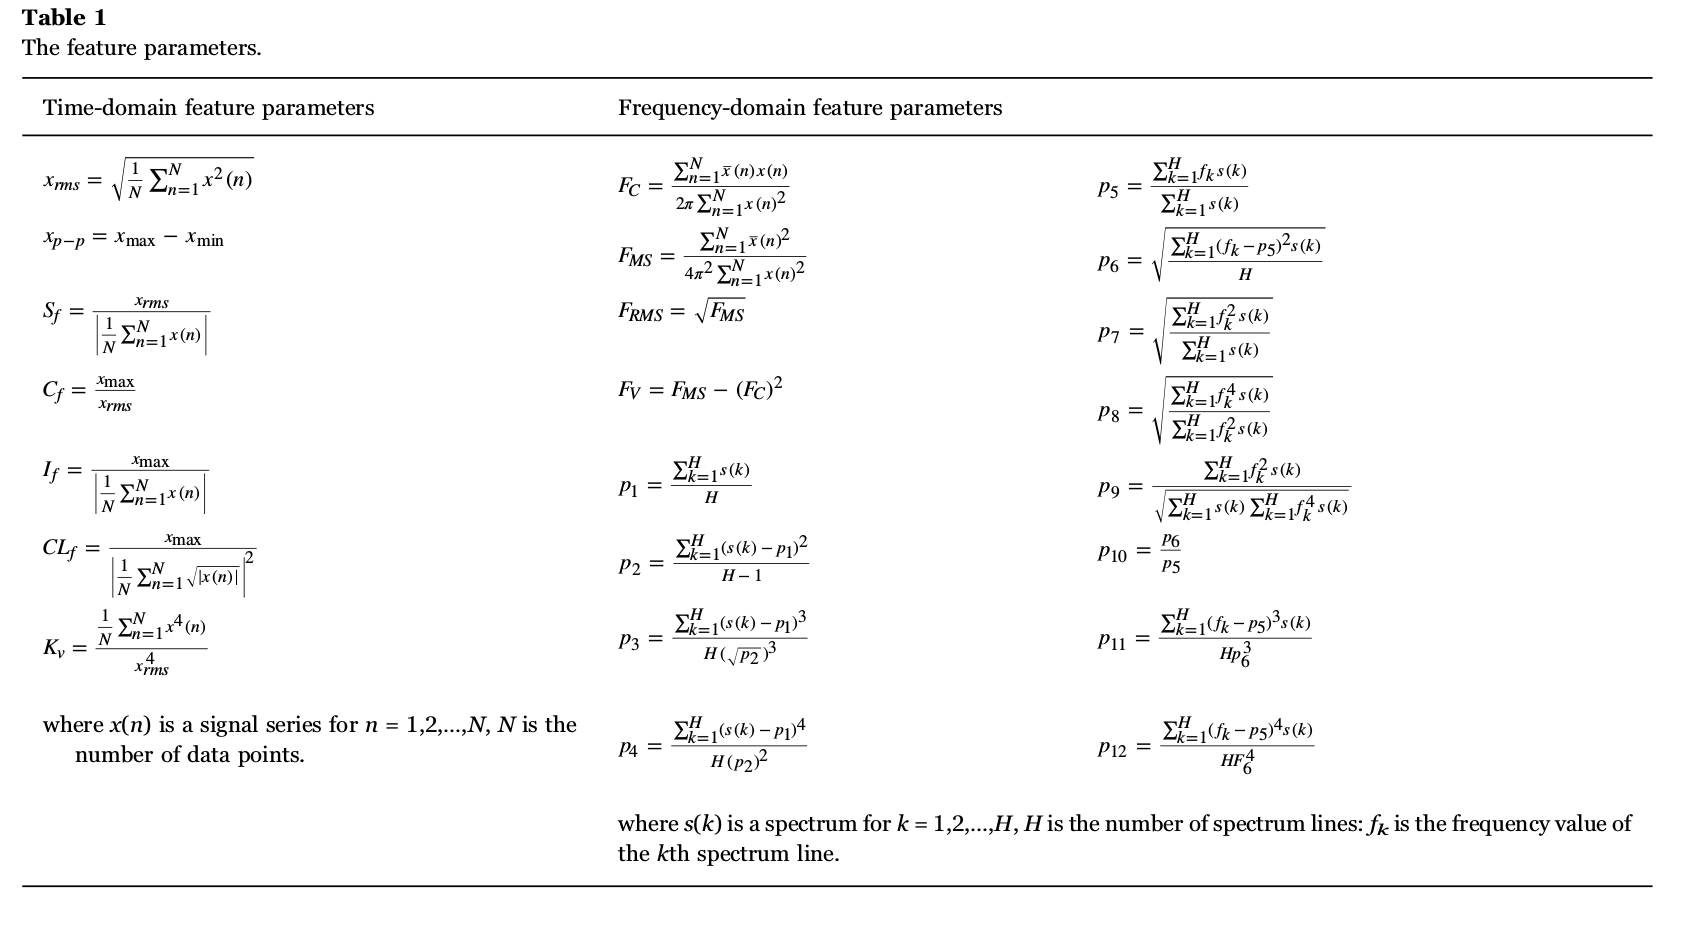
\includegraphics{attachment:image.png}
\end{figure}

    Entonces ahora definimos los features en el dominio del tiempo que
hallaremos para cada serie temporal

    \begin{Verbatim}[commandchars=\\\{\}]
{\color{incolor}In [{\color{incolor}11}]:} \PY{c+c1}{\PYZsh{}En todas las funciones x es un array que representa un time\PYZhy{}serie}
         \PY{k}{def} \PY{n+nf}{get\PYZus{}x\PYZus{}rms}\PY{p}{(}\PY{n}{x}\PY{p}{)}\PY{p}{:}
             \PY{n}{N}\PY{o}{=}\PY{n}{x}\PY{o}{.}\PY{n}{shape}\PY{p}{[}\PY{l+m+mi}{0}\PY{p}{]}
             \PY{k}{return} \PY{n}{np}\PY{o}{.}\PY{n}{power}\PY{p}{(}\PY{p}{(}\PY{n}{np}\PY{o}{.}\PY{n}{sum}\PY{p}{(}\PY{n}{np}\PY{o}{.}\PY{n}{power}\PY{p}{(}\PY{n}{x}\PY{p}{,} \PY{l+m+mi}{2}\PY{p}{)}\PY{p}{)}\PY{p}{)}\PY{o}{/}\PY{n}{N}\PY{p}{,} \PY{l+m+mf}{0.5}\PY{p}{)}

         \PY{k}{def} \PY{n+nf}{get\PYZus{}x\PYZus{}p\PYZus{}p}\PY{p}{(}\PY{n}{x}\PY{p}{)}\PY{p}{:}
             \PY{k}{return} \PY{n}{x}\PY{o}{.}\PY{n}{max}\PY{p}{(}\PY{p}{)}\PY{o}{\PYZhy{}}\PY{n}{x}\PY{o}{.}\PY{n}{min}\PY{p}{(}\PY{p}{)}

         \PY{k}{def} \PY{n+nf}{get\PYZus{}S\PYZus{}f}\PY{p}{(}\PY{n}{x}\PY{p}{)}\PY{p}{:}
             \PY{n}{N}\PY{o}{=}\PY{n}{x}\PY{o}{.}\PY{n}{shape}\PY{p}{[}\PY{l+m+mi}{0}\PY{p}{]}
             \PY{k}{return} \PY{n}{np}\PY{o}{.}\PY{n}{power}\PY{p}{(}\PY{p}{(}\PY{n}{np}\PY{o}{.}\PY{n}{sum}\PY{p}{(}\PY{n}{np}\PY{o}{.}\PY{n}{power}\PY{p}{(}\PY{n}{x}\PY{p}{,} \PY{l+m+mi}{2}\PY{p}{)}\PY{p}{)}\PY{p}{)}\PY{o}{/}\PY{n}{N}\PY{p}{,} \PY{l+m+mf}{0.5}\PY{p}{)}\PY{o}{/}\PY{n+nb}{abs}\PY{p}{(}\PY{n}{np}\PY{o}{.}\PY{n}{sum}\PY{p}{(}\PY{n}{x}\PY{p}{)}\PY{o}{/}\PY{n}{N}\PY{p}{)}

         \PY{k}{def} \PY{n+nf}{get\PYZus{}C\PYZus{}f}\PY{p}{(}\PY{n}{x}\PY{p}{)}\PY{p}{:}
             \PY{n}{N}\PY{o}{=}\PY{n}{x}\PY{o}{.}\PY{n}{shape}\PY{p}{[}\PY{l+m+mi}{0}\PY{p}{]}
             \PY{k}{return} \PY{n}{x}\PY{o}{.}\PY{n}{max}\PY{p}{(}\PY{p}{)}\PY{o}{/}\PY{n}{np}\PY{o}{.}\PY{n}{power}\PY{p}{(}\PY{p}{(}\PY{n}{np}\PY{o}{.}\PY{n}{sum}\PY{p}{(}\PY{n}{np}\PY{o}{.}\PY{n}{power}\PY{p}{(}\PY{n}{x}\PY{p}{,} \PY{l+m+mi}{2}\PY{p}{)}\PY{p}{)}\PY{p}{)}\PY{o}{/}\PY{n}{N}\PY{p}{,} \PY{l+m+mf}{0.5}\PY{p}{)}

         \PY{k}{def} \PY{n+nf}{get\PYZus{}I\PYZus{}f}\PY{p}{(}\PY{n}{x}\PY{p}{)}\PY{p}{:}
             \PY{n}{N}\PY{o}{=}\PY{n}{x}\PY{o}{.}\PY{n}{shape}\PY{p}{[}\PY{l+m+mi}{0}\PY{p}{]}
             \PY{k}{return} \PY{n}{x}\PY{o}{.}\PY{n}{max}\PY{p}{(}\PY{p}{)}\PY{o}{/}\PY{n+nb}{abs}\PY{p}{(}\PY{n}{np}\PY{o}{.}\PY{n}{sum}\PY{p}{(}\PY{n}{x}\PY{p}{)}\PY{o}{/}\PY{n}{N}\PY{p}{)}

         \PY{k}{def} \PY{n+nf}{get\PYZus{}CL\PYZus{}f}\PY{p}{(}\PY{n}{x}\PY{p}{)}\PY{p}{:}
             \PY{n}{N}\PY{o}{=}\PY{n}{x}\PY{o}{.}\PY{n}{shape}\PY{p}{[}\PY{l+m+mi}{0}\PY{p}{]}
             \PY{k}{return} \PY{n}{x}\PY{o}{.}\PY{n}{max}\PY{p}{(}\PY{p}{)}\PY{o}{/}\PY{n}{np}\PY{o}{.}\PY{n}{power}\PY{p}{(}\PY{n}{np}\PY{o}{.}\PY{n}{sum}\PY{p}{(}\PY{n}{np}\PY{o}{.}\PY{n}{power}\PY{p}{(}\PY{n+nb}{abs}\PY{p}{(}\PY{n}{x}\PY{p}{)}\PY{p}{,}\PY{l+m+mf}{0.5}\PY{p}{)}\PY{p}{)}\PY{o}{/}\PY{n}{N}\PY{p}{,}\PY{l+m+mi}{2}\PY{p}{)}

         \PY{k}{def} \PY{n+nf}{get\PYZus{}K\PYZus{}v}\PY{p}{(}\PY{n}{x}\PY{p}{)}\PY{p}{:}
             \PY{n}{N}\PY{o}{=}\PY{n}{x}\PY{o}{.}\PY{n}{shape}\PY{p}{[}\PY{l+m+mi}{0}\PY{p}{]}
             \PY{k}{return} \PY{n}{np}\PY{o}{.}\PY{n}{sum}\PY{p}{(}\PY{n}{np}\PY{o}{.}\PY{n}{power}\PY{p}{(}\PY{n}{x}\PY{p}{,}\PY{l+m+mi}{4}\PY{p}{)}\PY{p}{)}\PY{o}{/}\PY{p}{(}\PY{n}{np}\PY{o}{.}\PY{n}{power}\PY{p}{(}\PY{p}{(}\PY{n}{np}\PY{o}{.}\PY{n}{sum}\PY{p}{(}\PY{n}{np}\PY{o}{.}\PY{n}{power}\PY{p}{(}\PY{n}{x}\PY{p}{,} \PY{l+m+mi}{2}\PY{p}{)}\PY{p}{)}\PY{p}{)}\PY{o}{/}\PY{n}{N}\PY{p}{,} \PY{l+m+mi}{2}\PY{p}{)}\PY{o}{*}\PY{n}{N}\PY{p}{)}


         \PY{c+c1}{\PYZsh{} df: Es el dataframe cuyas columnas son los time\PYZhy{}series de los que se quiere}
         \PY{c+c1}{\PYZsh{} extraer los features}
         \PY{k}{def} \PY{n+nf}{get\PYZus{}features}\PY{p}{(}\PY{n}{df}\PY{p}{,}\PY{n}{col\PYZus{}prefix}\PY{o}{=}\PY{k+kc}{None}\PY{p}{)}\PY{p}{:}
             \PY{n}{col\PYZus{}sufix}\PY{o}{=}\PY{p}{[}\PY{l+s+s1}{\PYZsq{}}\PY{l+s+s1}{x\PYZus{}rms}\PY{l+s+s1}{\PYZsq{}}\PY{p}{,}\PY{l+s+s1}{\PYZsq{}}\PY{l+s+s1}{x\PYZus{}p\PYZus{}p}\PY{l+s+s1}{\PYZsq{}}\PY{p}{,}\PY{l+s+s1}{\PYZsq{}}\PY{l+s+s1}{S\PYZus{}f}\PY{l+s+s1}{\PYZsq{}}\PY{p}{,}\PY{l+s+s1}{\PYZsq{}}\PY{l+s+s1}{C\PYZus{}f}\PY{l+s+s1}{\PYZsq{}}\PY{p}{,}\PY{l+s+s1}{\PYZsq{}}\PY{l+s+s1}{I\PYZus{}f}\PY{l+s+s1}{\PYZsq{}}\PY{p}{,}\PY{l+s+s1}{\PYZsq{}}\PY{l+s+s1}{CL\PYZus{}f}\PY{l+s+s1}{\PYZsq{}}\PY{p}{,}\PY{l+s+s1}{\PYZsq{}}\PY{l+s+s1}{K\PYZus{}v}\PY{l+s+s1}{\PYZsq{}}\PY{p}{]}

             \PY{n}{x\PYZus{}rms\PYZus{}array}\PY{o}{=}\PY{p}{[}\PY{p}{]}
             \PY{n}{x\PYZus{}p\PYZus{}p\PYZus{}array}\PY{o}{=}\PY{p}{[}\PY{p}{]}
             \PY{n}{S\PYZus{}f\PYZus{}array}\PY{o}{=}\PY{p}{[}\PY{p}{]}
             \PY{n}{C\PYZus{}f\PYZus{}array}\PY{o}{=}\PY{p}{[}\PY{p}{]}
             \PY{n}{I\PYZus{}f\PYZus{}array}\PY{o}{=}\PY{p}{[}\PY{p}{]}
             \PY{n}{CL\PYZus{}f\PYZus{}array}\PY{o}{=}\PY{p}{[}\PY{p}{]}
             \PY{n}{K\PYZus{}v\PYZus{}array}\PY{o}{=}\PY{p}{[}\PY{p}{]}

             \PY{k}{for} \PY{n}{col} \PY{o+ow}{in} \PY{n+nb}{range}\PY{p}{(}\PY{n}{df}\PY{o}{.}\PY{n}{shape}\PY{p}{[}\PY{l+m+mi}{1}\PY{p}{]}\PY{p}{)}\PY{p}{:}
                 \PY{n}{x\PYZus{}rms\PYZus{}array}\PY{o}{.}\PY{n}{append}\PY{p}{(}\PY{n}{get\PYZus{}x\PYZus{}rms}\PY{p}{(}\PY{n}{df}\PY{o}{.}\PY{n}{iloc}\PY{p}{[}\PY{p}{:}\PY{p}{,}\PY{n}{col}\PY{p}{]}\PY{o}{.}\PY{n}{values}\PY{p}{)}\PY{p}{)}
                 \PY{n}{x\PYZus{}p\PYZus{}p\PYZus{}array}\PY{o}{.}\PY{n}{append}\PY{p}{(}\PY{n}{get\PYZus{}x\PYZus{}p\PYZus{}p}\PY{p}{(}\PY{n}{df}\PY{o}{.}\PY{n}{iloc}\PY{p}{[}\PY{p}{:}\PY{p}{,}\PY{n}{col}\PY{p}{]}\PY{o}{.}\PY{n}{values}\PY{p}{)}\PY{p}{)}
                 \PY{n}{S\PYZus{}f\PYZus{}array}\PY{o}{.}\PY{n}{append}\PY{p}{(}\PY{n}{get\PYZus{}S\PYZus{}f}\PY{p}{(}\PY{n}{df}\PY{o}{.}\PY{n}{iloc}\PY{p}{[}\PY{p}{:}\PY{p}{,}\PY{n}{col}\PY{p}{]}\PY{o}{.}\PY{n}{values}\PY{p}{)}\PY{p}{)}
                 \PY{n}{C\PYZus{}f\PYZus{}array}\PY{o}{.}\PY{n}{append}\PY{p}{(}\PY{n}{get\PYZus{}C\PYZus{}f}\PY{p}{(}\PY{n}{df}\PY{o}{.}\PY{n}{iloc}\PY{p}{[}\PY{p}{:}\PY{p}{,}\PY{n}{col}\PY{p}{]}\PY{o}{.}\PY{n}{values}\PY{p}{)}\PY{p}{)}
                 \PY{n}{I\PYZus{}f\PYZus{}array}\PY{o}{.}\PY{n}{append}\PY{p}{(}\PY{n}{get\PYZus{}I\PYZus{}f}\PY{p}{(}\PY{n}{df}\PY{o}{.}\PY{n}{iloc}\PY{p}{[}\PY{p}{:}\PY{p}{,}\PY{n}{col}\PY{p}{]}\PY{o}{.}\PY{n}{values}\PY{p}{)}\PY{p}{)}
                 \PY{n}{CL\PYZus{}f\PYZus{}array}\PY{o}{.}\PY{n}{append}\PY{p}{(}\PY{n}{get\PYZus{}CL\PYZus{}f}\PY{p}{(}\PY{n}{df}\PY{o}{.}\PY{n}{iloc}\PY{p}{[}\PY{p}{:}\PY{p}{,}\PY{n}{col}\PY{p}{]}\PY{o}{.}\PY{n}{values}\PY{p}{)}\PY{p}{)}
                 \PY{n}{K\PYZus{}v\PYZus{}array}\PY{o}{.}\PY{n}{append}\PY{p}{(}\PY{n}{get\PYZus{}K\PYZus{}v}\PY{p}{(}\PY{n}{df}\PY{o}{.}\PY{n}{iloc}\PY{p}{[}\PY{p}{:}\PY{p}{,}\PY{n}{col}\PY{p}{]}\PY{o}{.}\PY{n}{values}\PY{p}{)}\PY{p}{)}

             \PY{n}{features}\PY{o}{=}\PY{p}{[}\PY{n}{x\PYZus{}rms\PYZus{}array}\PY{p}{,}\PY{n}{x\PYZus{}p\PYZus{}p\PYZus{}array}\PY{p}{,}\PY{n}{S\PYZus{}f\PYZus{}array}\PY{p}{,}\PY{n}{C\PYZus{}f\PYZus{}array}\PY{p}{,}
                       \PY{n}{I\PYZus{}f\PYZus{}array}\PY{p}{,}\PY{n}{CL\PYZus{}f\PYZus{}array}\PY{p}{,}\PY{n}{K\PYZus{}v\PYZus{}array}\PY{p}{]}

             \PY{k}{if} \PY{n}{col\PYZus{}prefix}\PY{o}{==}\PY{k+kc}{None}\PY{p}{:}
                 \PY{n}{col\PYZus{}prefix}\PY{o}{=}\PY{n}{df}\PY{o}{.}\PY{n}{columns}

             \PY{n}{array\PYZus{}out}\PY{o}{=}\PY{p}{[}\PY{p}{]}
             \PY{n}{indexes}\PY{o}{=}\PY{p}{[}\PY{p}{]}
             \PY{k}{for} \PY{n}{col} \PY{o+ow}{in} \PY{n+nb}{range}\PY{p}{(}\PY{n}{df}\PY{o}{.}\PY{n}{shape}\PY{p}{[}\PY{l+m+mi}{1}\PY{p}{]}\PY{p}{)}\PY{p}{:}
                 \PY{k}{for} \PY{n}{feat} \PY{o+ow}{in} \PY{n+nb}{range}\PY{p}{(}\PY{l+m+mi}{7}\PY{p}{)}\PY{p}{:}
                     \PY{n}{indexes}\PY{o}{.}\PY{n}{append}\PY{p}{(}\PY{n}{col\PYZus{}prefix}\PY{p}{[}\PY{n}{col}\PY{p}{]}\PY{o}{+} \PY{l+s+s1}{\PYZsq{}}\PY{l+s+s1}{\PYZus{}}\PY{l+s+s1}{\PYZsq{}} \PY{o}{+} \PY{n}{col\PYZus{}sufix}\PY{p}{[}\PY{n}{feat}\PY{p}{]}\PY{p}{)}
                     \PY{n}{array\PYZus{}out}\PY{o}{.}\PY{n}{append}\PY{p}{(}\PY{n}{features}\PY{p}{[}\PY{n}{feat}\PY{p}{]}\PY{p}{[}\PY{n}{col}\PY{p}{]}\PY{p}{)}

             \PY{n}{series\PYZus{}out}\PY{o}{=}\PY{n}{pd}\PY{o}{.}\PY{n}{Series}\PY{p}{(}\PY{n}{array\PYZus{}out}\PY{p}{,}\PY{n}{indexes}\PY{p}{)}
             \PY{k}{return} \PY{n}{series\PYZus{}out}

         \PY{k}{def} \PY{n+nf}{concat\PYZus{}array\PYZus{}df}\PY{p}{(}\PY{n}{array\PYZus{}of\PYZus{}df}\PY{p}{)}\PY{p}{:}
             \PY{n}{df\PYZus{}out}\PY{o}{=}\PY{n}{array\PYZus{}of\PYZus{}df}\PY{p}{[}\PY{l+m+mi}{0}\PY{p}{]}\PY{o}{.}\PY{n}{copy}\PY{p}{(}\PY{p}{)}
             \PY{k}{for} \PY{n}{i} \PY{o+ow}{in} \PY{n+nb}{range}\PY{p}{(}\PY{l+m+mi}{1}\PY{p}{,}\PY{n+nb}{len}\PY{p}{(}\PY{n}{array\PYZus{}of\PYZus{}df}\PY{p}{)}\PY{p}{)}\PY{p}{:}
                 \PY{n}{df\PYZus{}out}\PY{o}{=}\PY{n}{pd}\PY{o}{.}\PY{n}{concat}\PY{p}{(}\PY{p}{[}\PY{n}{df\PYZus{}out}\PY{p}{,}\PY{n}{array\PYZus{}of\PYZus{}df}\PY{p}{[}\PY{n}{i}\PY{p}{]}\PY{p}{]}\PY{p}{,}\PY{n}{ignore\PYZus{}index}\PY{o}{=}\PY{k+kc}{True}\PY{p}{)}
             \PY{k}{return} \PY{n}{df\PYZus{}out}

         \PY{c+c1}{\PYZsh{} w: tamaño de ventana (número de filas)}
         \PY{c+c1}{\PYZsh{} Data: Lista en la que cada elemento es un Dataframe que representa a un archivo}
         \PY{c+c1}{\PYZsh{} columns: (Opcional) lista con los labels de las columnas que se quieren tener. }
         \PY{c+c1}{\PYZsh{}La última columna se asume como clase}
         \PY{k}{def} \PY{n+nf}{get\PYZus{}df\PYZus{}features\PYZus{}w}\PY{p}{(}\PY{n}{w}\PY{p}{,}\PY{n}{Data}\PY{p}{,}\PY{n}{columns}\PY{o}{=}\PY{k+kc}{None}\PY{p}{)}\PY{p}{:}
             \PY{n}{X\PYZus{}array}\PY{o}{=}\PY{p}{[}\PY{p}{]}
             \PY{n}{Y\PYZus{}array}\PY{o}{=}\PY{p}{[}\PY{p}{]}
             \PY{k}{if} \PY{n}{columns} \PY{o}{==} \PY{k+kc}{None}\PY{p}{:}
                 \PY{n}{columns}\PY{o}{=}\PY{n}{Data}\PY{p}{[}\PY{l+m+mi}{0}\PY{p}{]}\PY{o}{.}\PY{n}{columns}
             \PY{k}{for} \PY{n}{m} \PY{o+ow}{in} \PY{n+nb}{range}\PY{p}{(}\PY{n+nb}{len}\PY{p}{(}\PY{n}{Data}\PY{p}{)}\PY{p}{)}\PY{p}{:}
                 \PY{n}{row\PYZus{}index}\PY{o}{=}\PY{l+m+mi}{0}

                 \PY{k}{if} \PY{n}{Data}\PY{p}{[}\PY{n}{m}\PY{p}{]}\PY{o}{.}\PY{n}{shape}\PY{p}{[}\PY{l+m+mi}{0}\PY{p}{]}\PY{o}{\PYZgt{}}\PY{o}{=}\PY{n}{w}\PY{p}{:}
                     \PY{n}{rows\PYZus{}of\PYZus{}windows}\PY{o}{=}\PY{n}{math}\PY{o}{.}\PY{n}{floor}\PY{p}{(}\PY{n}{Data}\PY{p}{[}\PY{n}{m}\PY{p}{]}\PY{o}{.}\PY{n}{shape}\PY{p}{[}\PY{l+m+mi}{0}\PY{p}{]}\PY{o}{/}\PY{n}{w}\PY{p}{)}

                     \PY{k}{for} \PY{n}{n} \PY{o+ow}{in} \PY{n+nb}{range}\PY{p}{(}\PY{n}{rows\PYZus{}of\PYZus{}windows}\PY{p}{)}\PY{p}{:}
                         \PY{n}{Xdf\PYZus{}temp}\PY{o}{=}\PY{n}{Data}\PY{p}{[}\PY{n}{m}\PY{p}{]}\PY{p}{[}\PY{n}{columns}\PY{p}{]}\PY{o}{.}\PY{n}{iloc}\PY{p}{[}\PY{n}{row\PYZus{}index}\PY{p}{:}\PY{n}{row\PYZus{}index}\PY{o}{+}\PY{n}{w}\PY{p}{,}\PY{p}{:}\PY{o}{\PYZhy{}}\PY{l+m+mi}{1}\PY{p}{]}
                         \PY{c+c1}{\PYZsh{}Extraemos los features y ahora tenemos una fila por cada ventana w}
                         \PY{n}{Xdf\PYZus{}temp}\PY{o}{=}\PY{n}{get\PYZus{}features}\PY{p}{(}\PY{n}{Xdf\PYZus{}temp}\PY{p}{)}
                         \PY{n}{X\PYZus{}array}\PY{o}{.}\PY{n}{append}\PY{p}{(}\PY{n}{Xdf\PYZus{}temp}\PY{p}{)}

                         \PY{n}{Ydf\PYZus{}temp}\PY{o}{=}\PY{n}{Data}\PY{p}{[}\PY{n}{m}\PY{p}{]}\PY{o}{.}\PY{n}{iloc}\PY{p}{[}\PY{n}{row\PYZus{}index}\PY{p}{,}\PY{o}{\PYZhy{}}\PY{l+m+mi}{1}\PY{p}{]}\PY{c+c1}{\PYZsh{}Se toma solo el primer elemento }
                         \PY{c+c1}{\PYZsh{}porque la clase se repite y es la misma para cada archivo}
                         \PY{n}{Y\PYZus{}array}\PY{o}{.}\PY{n}{append}\PY{p}{(}\PY{n}{Ydf\PYZus{}temp}\PY{p}{)}
                         \PY{n}{row\PYZus{}index}\PY{o}{+}\PY{o}{=}\PY{n}{w}
                 \PY{k}{else}\PY{p}{:}
                     \PY{n+nb}{print}\PY{p}{(}\PY{l+s+s1}{\PYZsq{}}\PY{l+s+s1}{Tamaño de ventana w muy grande}\PY{l+s+s1}{\PYZsq{}}\PY{p}{)}

             \PY{n}{X\PYZus{}df}\PY{o}{=}\PY{n}{pd}\PY{o}{.}\PY{n}{DataFrame}\PY{p}{(}\PY{n}{X\PYZus{}array}\PY{p}{)}
             \PY{n}{Y\PYZus{}df}\PY{o}{=}\PY{n}{pd}\PY{o}{.}\PY{n}{DataFrame}\PY{p}{(}\PY{p}{\PYZob{}}\PY{l+s+s1}{\PYZsq{}}\PY{l+s+s1}{Rush}\PY{l+s+s1}{\PYZsq{}}\PY{p}{:}\PY{n}{Y\PYZus{}array}\PY{p}{\PYZcb{}}\PY{p}{)}
             \PY{k}{return} \PY{n}{X\PYZus{}df}\PY{p}{,}\PY{n}{Y\PYZus{}df}
\end{Verbatim}

    \begin{Verbatim}[commandchars=\\\{\}]
{\color{incolor}In [{\color{incolor}12}]:} \PY{n}{X\PYZus{}df}\PY{p}{,}\PY{n}{Y\PYZus{}df}\PY{o}{=}\PY{n}{get\PYZus{}df\PYZus{}features\PYZus{}w}\PY{p}{(}\PY{n}{w\PYZus{}max}\PY{p}{,}\PY{n}{Data}\PY{p}{,}\PY{p}{[}\PY{l+s+s1}{\PYZsq{}}\PY{l+s+s1}{Speed(m/s)}\PY{l+s+s1}{\PYZsq{}}\PY{p}{,}\PY{l+s+s1}{\PYZsq{}}\PY{l+s+s1}{Total\PYZus{}Acceleration(m/s\PYZca{}2)}\PY{l+s+s1}{\PYZsq{}}\PY{p}{,}
                                                 \PY{l+s+s1}{\PYZsq{}}\PY{l+s+s1}{Lateral\PYZus{}Acceleration(m/s\PYZca{}2)}\PY{l+s+s1}{\PYZsq{}}
                                             \PY{p}{,}\PY{l+s+s1}{\PYZsq{}}\PY{l+s+s1}{Engine RPM}\PY{l+s+s1}{\PYZsq{}}\PY{p}{,}\PY{l+s+s1}{\PYZsq{}}\PY{l+s+s1}{Pitch}\PY{l+s+s1}{\PYZsq{}}\PY{p}{,}\PY{l+s+s1}{\PYZsq{}}\PY{l+s+s1}{Driver\PYZus{}rush(0\PYZhy{}10)}\PY{l+s+s1}{\PYZsq{}}\PY{p}{]}\PY{p}{)}

         \PY{n}{Y\PYZus{}array}\PY{o}{=}\PY{n}{np}\PY{o}{.}\PY{n}{array}\PY{p}{(}\PY{p}{[}\PY{n+nb}{int}\PY{p}{(}\PY{n}{Y\PYZus{}df}\PY{o}{.}\PY{n}{values}\PY{p}{[}\PY{n}{i}\PY{p}{]}\PY{p}{)} \PY{k}{for} \PY{n}{i} \PY{o+ow}{in} \PY{n+nb}{range}\PY{p}{(}\PY{n}{Y\PYZus{}df}\PY{o}{.}\PY{n}{values}\PY{o}{.}\PY{n}{shape}\PY{p}{[}\PY{l+m+mi}{0}\PY{p}{]}\PY{p}{)}\PY{p}{]}\PY{p}{)}
         \PY{n+nb}{print}\PY{p}{(}\PY{n}{X\PYZus{}df}\PY{o}{.}\PY{n}{shape}\PY{p}{)}
         \PY{n+nb}{print}\PY{p}{(}\PY{n}{Y\PYZus{}df}\PY{o}{.}\PY{n}{shape}\PY{p}{)}
\end{Verbatim}

    \begin{Verbatim}[commandchars=\\\{\}]
(349, 35)
(349, 1)

    \end{Verbatim}

    Cómo se puede observar al elegir el tamaño de ventana máximo con \$
w=2000 \$ (de aproximada mente 20 s), se obtienen 3855 ventanas. Además
se extrajo los features de cada serie temporal (cada columna). Se
extrajeron 7 features y existían 5 columnas, por lo que se obtuvieron 35
columnas en el \emph{X\_df}

    \begin{Verbatim}[commandchars=\\\{\}]
{\color{incolor}In [{\color{incolor}13}]:} \PY{n}{X\PYZus{}df}\PY{p}{,}\PY{n}{Y\PYZus{}df}\PY{o}{=}\PY{n}{get\PYZus{}df\PYZus{}features\PYZus{}w}\PY{p}{(}\PY{l+m+mi}{2000}\PY{p}{,}\PY{n}{Data}\PY{p}{,}\PY{p}{[}\PY{l+s+s1}{\PYZsq{}}\PY{l+s+s1}{Speed(m/s)}\PY{l+s+s1}{\PYZsq{}}\PY{p}{,}\PY{l+s+s1}{\PYZsq{}}\PY{l+s+s1}{Total\PYZus{}Acceleration(m/s\PYZca{}2)}\PY{l+s+s1}{\PYZsq{}}\PY{p}{,}
                                                \PY{l+s+s1}{\PYZsq{}}\PY{l+s+s1}{Lateral\PYZus{}Acceleration(m/s\PYZca{}2)}\PY{l+s+s1}{\PYZsq{}}
                                                 \PY{p}{,}\PY{l+s+s1}{\PYZsq{}}\PY{l+s+s1}{Engine RPM}\PY{l+s+s1}{\PYZsq{}}\PY{p}{,}\PY{l+s+s1}{\PYZsq{}}\PY{l+s+s1}{Pitch}\PY{l+s+s1}{\PYZsq{}}\PY{p}{,}\PY{l+s+s1}{\PYZsq{}}\PY{l+s+s1}{Driver\PYZus{}rush(0\PYZhy{}10)}\PY{l+s+s1}{\PYZsq{}}\PY{p}{]}\PY{p}{)}
         \PY{n}{Y\PYZus{}array}\PY{o}{=}\PY{n}{np}\PY{o}{.}\PY{n}{array}\PY{p}{(}\PY{p}{[}\PY{n+nb}{int}\PY{p}{(}\PY{n}{Y\PYZus{}df}\PY{o}{.}\PY{n}{values}\PY{p}{[}\PY{n}{i}\PY{p}{]}\PY{p}{)} \PY{k}{for} \PY{n}{i} \PY{o+ow}{in} \PY{n+nb}{range}\PY{p}{(}\PY{n}{Y\PYZus{}df}\PY{o}{.}\PY{n}{values}\PY{o}{.}\PY{n}{shape}\PY{p}{[}\PY{l+m+mi}{0}\PY{p}{]}\PY{p}{)}\PY{p}{]}\PY{p}{)}
         \PY{n+nb}{print}\PY{p}{(}\PY{n}{X\PYZus{}df}\PY{o}{.}\PY{n}{shape}\PY{p}{)}
         \PY{n+nb}{print}\PY{p}{(}\PY{n}{Y\PYZus{}df}\PY{o}{.}\PY{n}{shape}\PY{p}{)}
\end{Verbatim}

    \begin{Verbatim}[commandchars=\\\{\}]
(3855, 35)
(3855, 1)

    \end{Verbatim}

    \subsection{5. Selección de
parámetros}\label{selecciuxf3n-de-paruxe1metros}

Ahora seleccionaremos sólo los parámetros que sean relevantes para la
clasificación. Para eso utilizaremos el algoritmo PCA para reucir a 4
componentes.

    \subsection{PCA}\label{pca}

    \begin{Verbatim}[commandchars=\\\{\}]
{\color{incolor}In [{\color{incolor}14}]:} \PY{k+kn}{from} \PY{n+nn}{sklearn}\PY{n+nn}{.}\PY{n+nn}{decomposition} \PY{k}{import} \PY{n}{PCA}
         \PY{n}{n\PYZus{}comp}\PY{o}{=}\PY{l+m+mi}{4}
         \PY{n}{PCA\PYZus{}obj} \PY{o}{=} \PY{n}{PCA}\PY{p}{(}\PY{n}{n\PYZus{}components} \PY{o}{=} \PY{n}{n\PYZus{}comp}\PY{p}{)}
         \PY{n}{X\PYZus{}reduct} \PY{o}{=} \PY{n}{PCA\PYZus{}obj}\PY{o}{.}\PY{n}{fit\PYZus{}transform}\PY{p}{(}\PY{n}{X\PYZus{}df}\PY{p}{)}
         \PY{n+nb}{print}\PY{p}{(}\PY{n}{X\PYZus{}reduct}\PY{o}{.}\PY{n}{shape}\PY{p}{)}
         \PY{n}{sns}\PY{o}{.}\PY{n}{set}\PY{p}{(}\PY{n}{font\PYZus{}scale}\PY{o}{=}\PY{l+m+mf}{1.3}\PY{p}{)}

         \PY{n}{variance}\PY{o}{=}\PY{n}{PCA\PYZus{}obj}\PY{o}{.}\PY{n}{explained\PYZus{}variance\PYZus{}ratio\PYZus{}}
         \PY{n}{variance}\PY{o}{=}\PY{p}{[}\PY{n}{variance}\PY{p}{[}\PY{n}{i}\PY{p}{]}\PY{o}{*}\PY{l+m+mi}{100} \PY{k}{for} \PY{n}{i} \PY{o+ow}{in} \PY{n+nb}{range}\PY{p}{(}\PY{n}{variance}\PY{o}{.}\PY{n}{shape}\PY{p}{[}\PY{l+m+mi}{0}\PY{p}{]}\PY{p}{)}\PY{p}{]}
         \PY{n}{fig1}\PY{o}{=} \PY{n}{plt}\PY{o}{.}\PY{n}{figure}\PY{p}{(}\PY{n}{figsize}\PY{o}{=}\PY{p}{(}\PY{l+m+mi}{13}\PY{p}{,}\PY{l+m+mi}{5}\PY{p}{)}\PY{p}{,} \PY{n}{dpi}\PY{o}{=}\PY{l+m+mi}{100}\PY{p}{)}
         \PY{n}{graph}\PY{o}{=}\PY{n}{sns}\PY{o}{.}\PY{n}{barplot}\PY{p}{(}\PY{n}{variance}\PY{p}{,}\PY{n+nb}{list}\PY{p}{(}\PY{n+nb}{range}\PY{p}{(}\PY{l+m+mi}{1}\PY{p}{,}\PY{n}{n\PYZus{}comp}\PY{o}{+}\PY{l+m+mi}{1}\PY{p}{)}\PY{p}{)}\PY{p}{,} \PY{n}{orient}\PY{o}{=}\PY{l+s+s1}{\PYZsq{}}\PY{l+s+s1}{h}\PY{l+s+s1}{\PYZsq{}}\PY{p}{)}
         \PY{n}{plt}\PY{o}{.}\PY{n}{ylabel}\PY{p}{(}\PY{l+s+s1}{\PYZsq{}}\PY{l+s+s1}{Número de componente}\PY{l+s+s1}{\PYZsq{}}\PY{p}{)}
         \PY{n}{plt}\PY{o}{.}\PY{n}{xlabel}\PY{p}{(}\PY{l+s+s1}{\PYZsq{}}\PY{l+s+s1}{Porcentaje (}\PY{l+s+s1}{\PYZpc{}}\PY{l+s+s1}{)}\PY{l+s+s1}{\PYZsq{}}\PY{p}{)}
         \PY{n}{plt}\PY{o}{.}\PY{n}{xlim}\PY{p}{(}\PY{p}{[}\PY{l+m+mi}{0}\PY{p}{,} \PY{l+m+mi}{80}\PY{p}{]}\PY{p}{)}

         \PY{k}{for} \PY{n}{i}\PY{p}{,} \PY{n}{v} \PY{o+ow}{in} \PY{n+nb}{enumerate}\PY{p}{(}\PY{n}{variance}\PY{p}{)}\PY{p}{:}
             \PY{n}{graph}\PY{o}{.}\PY{n}{text}\PY{p}{(}\PY{n}{v} \PY{o}{+}\PY{l+m+mf}{0.3}\PY{p}{,} \PY{n}{i} \PY{p}{,} \PY{n+nb}{str}\PY{p}{(}\PY{n+nb}{round}\PY{p}{(}\PY{n}{v}\PY{p}{,}\PY{l+m+mi}{2}\PY{p}{)}\PY{p}{)}\PY{o}{+}\PY{l+s+s1}{\PYZsq{}}\PY{l+s+s1}{\PYZpc{}}\PY{l+s+s1}{\PYZsq{}}\PY{p}{,} \PY{n}{color}\PY{o}{=}\PY{l+s+s1}{\PYZsq{}}\PY{l+s+s1}{black}\PY{l+s+s1}{\PYZsq{}}\PY{p}{,} \PY{n}{fontweight}\PY{o}{=}\PY{l+s+s1}{\PYZsq{}}\PY{l+s+s1}{bold}\PY{l+s+s1}{\PYZsq{}}\PY{p}{)}

         \PY{n}{fig1}\PY{o}{.}\PY{n}{savefig}\PY{p}{(}\PY{l+s+s2}{\PYZdq{}}\PY{l+s+s2}{./Figuras/PCA\PYZus{}dist.pdf}\PY{l+s+s2}{\PYZdq{}}\PY{p}{,} \PY{n}{bbox\PYZus{}inches}\PY{o}{=}\PY{l+s+s1}{\PYZsq{}}\PY{l+s+s1}{tight}\PY{l+s+s1}{\PYZsq{}}\PY{p}{)}
\end{Verbatim}

    \begin{Verbatim}[commandchars=\\\{\}]
(3855, 4)

    \end{Verbatim}

    \begin{center}
    \adjustimage{max size={0.9\linewidth}{0.9\paperheight}}{output_31_1.png}
    \end{center}
    { \hspace*{\fill} \\}

    \begin{Verbatim}[commandchars=\\\{\}]
{\color{incolor}In [{\color{incolor}15}]:} \PY{n}{fig}\PY{p}{,} \PY{n}{axes} \PY{o}{=} \PY{n}{plt}\PY{o}{.}\PY{n}{subplots}\PY{p}{(}\PY{l+m+mi}{3}\PY{p}{,} \PY{l+m+mi}{2}\PY{p}{,}\PY{n}{figsize}\PY{o}{=}\PY{p}{(}\PY{l+m+mi}{15}\PY{p}{,}\PY{l+m+mi}{17}\PY{p}{)}\PY{p}{)}
         \PY{n}{axes}\PY{p}{[}\PY{l+m+mi}{0}\PY{p}{,} \PY{l+m+mi}{0}\PY{p}{]}\PY{o}{.}\PY{n}{scatter}\PY{p}{(}\PY{n}{X\PYZus{}reduct}\PY{p}{[}\PY{p}{:}\PY{p}{,}\PY{l+m+mi}{0}\PY{p}{]}\PY{p}{,} \PY{n}{X\PYZus{}reduct}\PY{p}{[}\PY{p}{:}\PY{p}{,}\PY{l+m+mi}{1}\PY{p}{]}\PY{p}{,} \PY{n}{c}\PY{o}{=}\PY{n}{Y\PYZus{}array}\PY{p}{,} \PY{n}{cmap}\PY{o}{=}\PY{n}{plt}\PY{o}{.}\PY{n}{cm}\PY{o}{.}\PY{n}{rainbow}\PY{p}{)}
         \PY{n}{axes}\PY{p}{[}\PY{l+m+mi}{0}\PY{p}{,} \PY{l+m+mi}{0}\PY{p}{]}\PY{o}{.}\PY{n}{set\PYZus{}title}\PY{p}{(}\PY{l+s+s1}{\PYZsq{}}\PY{l+s+s1}{Componente 1 vs 2}\PY{l+s+s1}{\PYZsq{}}\PY{p}{)}
         \PY{c+c1}{\PYZsh{} plt.ylabel(\PYZsq{}Componente 2\PYZsq{})}
         \PY{c+c1}{\PYZsh{} plt.xlabel(\PYZsq{}Componente 1\PYZsq{})}

         \PY{n}{axes}\PY{p}{[}\PY{l+m+mi}{0}\PY{p}{,} \PY{l+m+mi}{1}\PY{p}{]}\PY{o}{.}\PY{n}{scatter}\PY{p}{(}\PY{n}{X\PYZus{}reduct}\PY{p}{[}\PY{p}{:}\PY{p}{,}\PY{l+m+mi}{0}\PY{p}{]}\PY{p}{,} \PY{n}{X\PYZus{}reduct}\PY{p}{[}\PY{p}{:}\PY{p}{,}\PY{l+m+mi}{2}\PY{p}{]}\PY{p}{,} \PY{n}{c}\PY{o}{=}\PY{n}{Y\PYZus{}array}\PY{p}{,} \PY{n}{cmap}\PY{o}{=}\PY{n}{plt}\PY{o}{.}\PY{n}{cm}\PY{o}{.}\PY{n}{rainbow}\PY{p}{)}
         \PY{n}{axes}\PY{p}{[}\PY{l+m+mi}{0}\PY{p}{,} \PY{l+m+mi}{1}\PY{p}{]}\PY{o}{.}\PY{n}{set\PYZus{}title}\PY{p}{(}\PY{l+s+s1}{\PYZsq{}}\PY{l+s+s1}{Componente 1 vs 3}\PY{l+s+s1}{\PYZsq{}}\PY{p}{)}
         \PY{c+c1}{\PYZsh{} plt.ylabel(\PYZsq{}Componente 3\PYZsq{})}
         \PY{c+c1}{\PYZsh{} plt.xlabel(\PYZsq{}Componente 1\PYZsq{})}

         \PY{n}{axes}\PY{p}{[}\PY{l+m+mi}{1}\PY{p}{,} \PY{l+m+mi}{0}\PY{p}{]}\PY{o}{.}\PY{n}{scatter}\PY{p}{(}\PY{n}{X\PYZus{}reduct}\PY{p}{[}\PY{p}{:}\PY{p}{,}\PY{l+m+mi}{0}\PY{p}{]}\PY{p}{,} \PY{n}{X\PYZus{}reduct}\PY{p}{[}\PY{p}{:}\PY{p}{,}\PY{l+m+mi}{3}\PY{p}{]}\PY{p}{,} \PY{n}{c}\PY{o}{=}\PY{n}{Y\PYZus{}array}\PY{p}{,} \PY{n}{cmap}\PY{o}{=}\PY{n}{plt}\PY{o}{.}\PY{n}{cm}\PY{o}{.}\PY{n}{rainbow}\PY{p}{)}
         \PY{n}{axes}\PY{p}{[}\PY{l+m+mi}{1}\PY{p}{,} \PY{l+m+mi}{0}\PY{p}{]}\PY{o}{.}\PY{n}{set\PYZus{}title}\PY{p}{(}\PY{l+s+s1}{\PYZsq{}}\PY{l+s+s1}{Componente 1 vs 4}\PY{l+s+s1}{\PYZsq{}}\PY{p}{)}
         \PY{c+c1}{\PYZsh{} plt.ylabel(\PYZsq{}Componente 4\PYZsq{})}
         \PY{c+c1}{\PYZsh{} plt.xlabel(\PYZsq{}Componente 1\PYZsq{})}

         \PY{n}{axes}\PY{p}{[}\PY{l+m+mi}{1}\PY{p}{,} \PY{l+m+mi}{1}\PY{p}{]}\PY{o}{.}\PY{n}{scatter}\PY{p}{(}\PY{n}{X\PYZus{}reduct}\PY{p}{[}\PY{p}{:}\PY{p}{,}\PY{l+m+mi}{1}\PY{p}{]}\PY{p}{,} \PY{n}{X\PYZus{}reduct}\PY{p}{[}\PY{p}{:}\PY{p}{,}\PY{l+m+mi}{2}\PY{p}{]}\PY{p}{,} \PY{n}{c}\PY{o}{=}\PY{n}{Y\PYZus{}array}\PY{p}{,} \PY{n}{cmap}\PY{o}{=}\PY{n}{plt}\PY{o}{.}\PY{n}{cm}\PY{o}{.}\PY{n}{rainbow}\PY{p}{)}
         \PY{n}{axes}\PY{p}{[}\PY{l+m+mi}{1}\PY{p}{,} \PY{l+m+mi}{1}\PY{p}{]}\PY{o}{.}\PY{n}{set\PYZus{}title}\PY{p}{(}\PY{l+s+s1}{\PYZsq{}}\PY{l+s+s1}{Componente 2 vs 3}\PY{l+s+s1}{\PYZsq{}}\PY{p}{)}
         \PY{c+c1}{\PYZsh{} plt.ylabel(\PYZsq{}Componente 3\PYZsq{})}
         \PY{c+c1}{\PYZsh{} plt.xlabel(\PYZsq{}Componente 2\PYZsq{})}

         \PY{n}{axes}\PY{p}{[}\PY{l+m+mi}{2}\PY{p}{,} \PY{l+m+mi}{0}\PY{p}{]}\PY{o}{.}\PY{n}{scatter}\PY{p}{(}\PY{n}{X\PYZus{}reduct}\PY{p}{[}\PY{p}{:}\PY{p}{,}\PY{l+m+mi}{1}\PY{p}{]}\PY{p}{,} \PY{n}{X\PYZus{}reduct}\PY{p}{[}\PY{p}{:}\PY{p}{,}\PY{l+m+mi}{3}\PY{p}{]}\PY{p}{,} \PY{n}{c}\PY{o}{=}\PY{n}{Y\PYZus{}array}\PY{p}{,} \PY{n}{cmap}\PY{o}{=}\PY{n}{plt}\PY{o}{.}\PY{n}{cm}\PY{o}{.}\PY{n}{rainbow}\PY{p}{)}
         \PY{n}{axes}\PY{p}{[}\PY{l+m+mi}{2}\PY{p}{,} \PY{l+m+mi}{0}\PY{p}{]}\PY{o}{.}\PY{n}{set\PYZus{}title}\PY{p}{(}\PY{l+s+s1}{\PYZsq{}}\PY{l+s+s1}{Componente 2 vs 4}\PY{l+s+s1}{\PYZsq{}}\PY{p}{)}
         \PY{c+c1}{\PYZsh{} plt.ylabel(\PYZsq{}Componente 4\PYZsq{})}
         \PY{c+c1}{\PYZsh{} plt.xlabel(\PYZsq{}Componente 2\PYZsq{})}

         \PY{n}{axes}\PY{p}{[}\PY{l+m+mi}{2}\PY{p}{,} \PY{l+m+mi}{1}\PY{p}{]}\PY{o}{.}\PY{n}{scatter}\PY{p}{(}\PY{n}{X\PYZus{}reduct}\PY{p}{[}\PY{p}{:}\PY{p}{,}\PY{l+m+mi}{2}\PY{p}{]}\PY{p}{,} \PY{n}{X\PYZus{}reduct}\PY{p}{[}\PY{p}{:}\PY{p}{,}\PY{l+m+mi}{3}\PY{p}{]}\PY{p}{,} \PY{n}{c}\PY{o}{=}\PY{n}{Y\PYZus{}array}\PY{p}{,} \PY{n}{cmap}\PY{o}{=}\PY{n}{plt}\PY{o}{.}\PY{n}{cm}\PY{o}{.}\PY{n}{rainbow}\PY{p}{)}
         \PY{n}{axes}\PY{p}{[}\PY{l+m+mi}{2}\PY{p}{,} \PY{l+m+mi}{1}\PY{p}{]}\PY{o}{.}\PY{n}{set\PYZus{}title}\PY{p}{(}\PY{l+s+s1}{\PYZsq{}}\PY{l+s+s1}{Componente 3 vs 4}\PY{l+s+s1}{\PYZsq{}}\PY{p}{)}
         \PY{c+c1}{\PYZsh{} plt.ylabel(\PYZsq{}Componente 4\PYZsq{})}
         \PY{c+c1}{\PYZsh{} plt.xlabel(\PYZsq{}Componente 3\PYZsq{})}

         \PY{n}{plt}\PY{o}{.}\PY{n}{subplots\PYZus{}adjust}\PY{p}{(}\PY{n}{hspace}\PY{o}{=}\PY{l+m+mf}{0.3}\PY{p}{)}

         \PY{n}{fig}\PY{o}{.}\PY{n}{savefig}\PY{p}{(}\PY{l+s+s2}{\PYZdq{}}\PY{l+s+s2}{./Figuras/PCA\PYZus{}vs.pdf}\PY{l+s+s2}{\PYZdq{}}\PY{p}{,} \PY{n}{bbox\PYZus{}inches}\PY{o}{=}\PY{l+s+s1}{\PYZsq{}}\PY{l+s+s1}{tight}\PY{l+s+s1}{\PYZsq{}}\PY{p}{)}
\end{Verbatim}

    \begin{center}
    \adjustimage{max size={0.9\linewidth}{0.9\paperheight}}{output_32_0.png}
    \end{center}
    { \hspace*{\fill} \\}

    Se usa FastICA para intentar separar loc componentes seleccionados

    \begin{Verbatim}[commandchars=\\\{\}]
{\color{incolor}In [{\color{incolor}16}]:} \PY{k+kn}{from} \PY{n+nn}{sklearn}\PY{n+nn}{.}\PY{n+nn}{decomposition} \PY{k}{import} \PY{n}{FastICA}
         \PY{n}{n\PYZus{}comp}\PY{o}{=}\PY{l+m+mi}{4}
         \PY{n}{FastICA\PYZus{}tr} \PY{o}{=} \PY{n}{FastICA}\PY{p}{(}\PY{n}{n\PYZus{}components}\PY{o}{=}\PY{n}{n\PYZus{}comp}\PY{p}{,} \PY{n}{random\PYZus{}state}\PY{o}{=}\PY{l+m+mi}{0}\PY{p}{,} \PY{n}{algorithm}\PY{o}{=}\PY{l+s+s1}{\PYZsq{}}\PY{l+s+s1}{deflation}\PY{l+s+s1}{\PYZsq{}}\PY{p}{)}
         \PY{n}{X\PYZus{}reduct3} \PY{o}{=} \PY{n}{FastICA\PYZus{}tr}\PY{o}{.}\PY{n}{fit\PYZus{}transform}\PY{p}{(}\PY{n}{X\PYZus{}reduct}\PY{p}{)}
         \PY{n}{X\PYZus{}reduct3}\PY{o}{.}\PY{n}{shape}
\end{Verbatim}

\begin{Verbatim}[commandchars=\\\{\}]
{\color{outcolor}Out[{\color{outcolor}16}]:} (3855, 4)
\end{Verbatim}

    \begin{Verbatim}[commandchars=\\\{\}]
{\color{incolor}In [{\color{incolor}17}]:} \PY{n}{fig}\PY{p}{,} \PY{n}{axes} \PY{o}{=} \PY{n}{plt}\PY{o}{.}\PY{n}{subplots}\PY{p}{(}\PY{l+m+mi}{3}\PY{p}{,} \PY{l+m+mi}{2}\PY{p}{,}\PY{n}{figsize}\PY{o}{=}\PY{p}{(}\PY{l+m+mi}{15}\PY{p}{,}\PY{l+m+mi}{17}\PY{p}{)}\PY{p}{)}
         \PY{n}{axes}\PY{p}{[}\PY{l+m+mi}{0}\PY{p}{,} \PY{l+m+mi}{0}\PY{p}{]}\PY{o}{.}\PY{n}{scatter}\PY{p}{(}\PY{n}{X\PYZus{}reduct3}\PY{p}{[}\PY{p}{:}\PY{p}{,}\PY{l+m+mi}{0}\PY{p}{]}\PY{p}{,} \PY{n}{X\PYZus{}reduct3}\PY{p}{[}\PY{p}{:}\PY{p}{,}\PY{l+m+mi}{1}\PY{p}{]}\PY{p}{,} \PY{n}{c}\PY{o}{=}\PY{n}{Y\PYZus{}array}\PY{p}{,} \PY{n}{cmap}\PY{o}{=}\PY{n}{plt}\PY{o}{.}\PY{n}{cm}\PY{o}{.}\PY{n}{rainbow}\PY{p}{)}
         \PY{n}{axes}\PY{p}{[}\PY{l+m+mi}{0}\PY{p}{,} \PY{l+m+mi}{0}\PY{p}{]}\PY{o}{.}\PY{n}{set\PYZus{}title}\PY{p}{(}\PY{l+s+s1}{\PYZsq{}}\PY{l+s+s1}{Componente 1 vs 2}\PY{l+s+s1}{\PYZsq{}}\PY{p}{)}
         \PY{c+c1}{\PYZsh{} plt.ylabel(\PYZsq{}Componente 2\PYZsq{})}
         \PY{c+c1}{\PYZsh{} plt.xlabel(\PYZsq{}Componente 1\PYZsq{})}

         \PY{n}{axes}\PY{p}{[}\PY{l+m+mi}{0}\PY{p}{,} \PY{l+m+mi}{1}\PY{p}{]}\PY{o}{.}\PY{n}{scatter}\PY{p}{(}\PY{n}{X\PYZus{}reduct3}\PY{p}{[}\PY{p}{:}\PY{p}{,}\PY{l+m+mi}{0}\PY{p}{]}\PY{p}{,} \PY{n}{X\PYZus{}reduct3}\PY{p}{[}\PY{p}{:}\PY{p}{,}\PY{l+m+mi}{2}\PY{p}{]}\PY{p}{,} \PY{n}{c}\PY{o}{=}\PY{n}{Y\PYZus{}array}\PY{p}{,} \PY{n}{cmap}\PY{o}{=}\PY{n}{plt}\PY{o}{.}\PY{n}{cm}\PY{o}{.}\PY{n}{rainbow}\PY{p}{)}
         \PY{n}{axes}\PY{p}{[}\PY{l+m+mi}{0}\PY{p}{,} \PY{l+m+mi}{1}\PY{p}{]}\PY{o}{.}\PY{n}{set\PYZus{}title}\PY{p}{(}\PY{l+s+s1}{\PYZsq{}}\PY{l+s+s1}{Componente 1 vs 3}\PY{l+s+s1}{\PYZsq{}}\PY{p}{)}
         \PY{c+c1}{\PYZsh{} plt.ylabel(\PYZsq{}Componente 3\PYZsq{})}
         \PY{c+c1}{\PYZsh{} plt.xlabel(\PYZsq{}Componente 1\PYZsq{})}

         \PY{n}{axes}\PY{p}{[}\PY{l+m+mi}{1}\PY{p}{,} \PY{l+m+mi}{0}\PY{p}{]}\PY{o}{.}\PY{n}{scatter}\PY{p}{(}\PY{n}{X\PYZus{}reduct3}\PY{p}{[}\PY{p}{:}\PY{p}{,}\PY{l+m+mi}{0}\PY{p}{]}\PY{p}{,} \PY{n}{X\PYZus{}reduct3}\PY{p}{[}\PY{p}{:}\PY{p}{,}\PY{l+m+mi}{3}\PY{p}{]}\PY{p}{,} \PY{n}{c}\PY{o}{=}\PY{n}{Y\PYZus{}array}\PY{p}{,} \PY{n}{cmap}\PY{o}{=}\PY{n}{plt}\PY{o}{.}\PY{n}{cm}\PY{o}{.}\PY{n}{rainbow}\PY{p}{)}
         \PY{n}{axes}\PY{p}{[}\PY{l+m+mi}{1}\PY{p}{,} \PY{l+m+mi}{0}\PY{p}{]}\PY{o}{.}\PY{n}{set\PYZus{}title}\PY{p}{(}\PY{l+s+s1}{\PYZsq{}}\PY{l+s+s1}{Componente 1 vs 4}\PY{l+s+s1}{\PYZsq{}}\PY{p}{)}
         \PY{c+c1}{\PYZsh{} plt.ylabel(\PYZsq{}Componente 4\PYZsq{})}
         \PY{c+c1}{\PYZsh{} plt.xlabel(\PYZsq{}Componente 1\PYZsq{})}

         \PY{n}{axes}\PY{p}{[}\PY{l+m+mi}{1}\PY{p}{,} \PY{l+m+mi}{1}\PY{p}{]}\PY{o}{.}\PY{n}{scatter}\PY{p}{(}\PY{n}{X\PYZus{}reduct3}\PY{p}{[}\PY{p}{:}\PY{p}{,}\PY{l+m+mi}{1}\PY{p}{]}\PY{p}{,} \PY{n}{X\PYZus{}reduct3}\PY{p}{[}\PY{p}{:}\PY{p}{,}\PY{l+m+mi}{2}\PY{p}{]}\PY{p}{,} \PY{n}{c}\PY{o}{=}\PY{n}{Y\PYZus{}array}\PY{p}{,} \PY{n}{cmap}\PY{o}{=}\PY{n}{plt}\PY{o}{.}\PY{n}{cm}\PY{o}{.}\PY{n}{rainbow}\PY{p}{)}
         \PY{n}{axes}\PY{p}{[}\PY{l+m+mi}{1}\PY{p}{,} \PY{l+m+mi}{1}\PY{p}{]}\PY{o}{.}\PY{n}{set\PYZus{}title}\PY{p}{(}\PY{l+s+s1}{\PYZsq{}}\PY{l+s+s1}{Componente 2 vs 3}\PY{l+s+s1}{\PYZsq{}}\PY{p}{)}
         \PY{c+c1}{\PYZsh{} plt.ylabel(\PYZsq{}Componente 3\PYZsq{})}
         \PY{c+c1}{\PYZsh{} plt.xlabel(\PYZsq{}Componente 2\PYZsq{})}

         \PY{n}{axes}\PY{p}{[}\PY{l+m+mi}{2}\PY{p}{,} \PY{l+m+mi}{0}\PY{p}{]}\PY{o}{.}\PY{n}{scatter}\PY{p}{(}\PY{n}{X\PYZus{}reduct3}\PY{p}{[}\PY{p}{:}\PY{p}{,}\PY{l+m+mi}{1}\PY{p}{]}\PY{p}{,} \PY{n}{X\PYZus{}reduct3}\PY{p}{[}\PY{p}{:}\PY{p}{,}\PY{l+m+mi}{3}\PY{p}{]}\PY{p}{,} \PY{n}{c}\PY{o}{=}\PY{n}{Y\PYZus{}array}\PY{p}{,} \PY{n}{cmap}\PY{o}{=}\PY{n}{plt}\PY{o}{.}\PY{n}{cm}\PY{o}{.}\PY{n}{rainbow}\PY{p}{)}
         \PY{n}{axes}\PY{p}{[}\PY{l+m+mi}{2}\PY{p}{,} \PY{l+m+mi}{0}\PY{p}{]}\PY{o}{.}\PY{n}{set\PYZus{}title}\PY{p}{(}\PY{l+s+s1}{\PYZsq{}}\PY{l+s+s1}{Componente 2 vs 4}\PY{l+s+s1}{\PYZsq{}}\PY{p}{)}
         \PY{c+c1}{\PYZsh{} plt.ylabel(\PYZsq{}Componente 4\PYZsq{})}
         \PY{c+c1}{\PYZsh{} plt.xlabel(\PYZsq{}Componente 2\PYZsq{})}

         \PY{n}{axes}\PY{p}{[}\PY{l+m+mi}{2}\PY{p}{,} \PY{l+m+mi}{1}\PY{p}{]}\PY{o}{.}\PY{n}{scatter}\PY{p}{(}\PY{n}{X\PYZus{}reduct3}\PY{p}{[}\PY{p}{:}\PY{p}{,}\PY{l+m+mi}{2}\PY{p}{]}\PY{p}{,} \PY{n}{X\PYZus{}reduct3}\PY{p}{[}\PY{p}{:}\PY{p}{,}\PY{l+m+mi}{3}\PY{p}{]}\PY{p}{,} \PY{n}{c}\PY{o}{=}\PY{n}{Y\PYZus{}array}\PY{p}{,} \PY{n}{cmap}\PY{o}{=}\PY{n}{plt}\PY{o}{.}\PY{n}{cm}\PY{o}{.}\PY{n}{rainbow}\PY{p}{)}
         \PY{n}{axes}\PY{p}{[}\PY{l+m+mi}{2}\PY{p}{,} \PY{l+m+mi}{1}\PY{p}{]}\PY{o}{.}\PY{n}{set\PYZus{}title}\PY{p}{(}\PY{l+s+s1}{\PYZsq{}}\PY{l+s+s1}{Componente 3 vs 4}\PY{l+s+s1}{\PYZsq{}}\PY{p}{)}
         \PY{c+c1}{\PYZsh{} plt.ylabel(\PYZsq{}Componente 4\PYZsq{})}
         \PY{c+c1}{\PYZsh{} plt.xlabel(\PYZsq{}Componente 3\PYZsq{})}

         \PY{n}{plt}\PY{o}{.}\PY{n}{subplots\PYZus{}adjust}\PY{p}{(}\PY{n}{hspace}\PY{o}{=}\PY{l+m+mf}{0.3}\PY{p}{)}

         \PY{n}{fig}\PY{o}{.}\PY{n}{savefig}\PY{p}{(}\PY{l+s+s2}{\PYZdq{}}\PY{l+s+s2}{./Figuras/PCA\PYZus{}vs\PYZus{}separados.pdf}\PY{l+s+s2}{\PYZdq{}}\PY{p}{,} \PY{n}{bbox\PYZus{}inches}\PY{o}{=}\PY{l+s+s1}{\PYZsq{}}\PY{l+s+s1}{tight}\PY{l+s+s1}{\PYZsq{}}\PY{p}{)}
\end{Verbatim}

    \begin{center}
    \adjustimage{max size={0.9\linewidth}{0.9\paperheight}}{output_35_0.png}
    \end{center}
    { \hspace*{\fill} \\}

    \subsection{Model training}\label{model-training}

\subsubsection{Splitting into train an test
datasets}\label{splitting-into-train-an-test-datasets}

    \begin{Verbatim}[commandchars=\\\{\}]
{\color{incolor}In [{\color{incolor}18}]:} \PY{n}{X\PYZus{}data}\PY{o}{=}\PY{n}{X\PYZus{}reduct3}
         \PY{n}{test\PYZus{}size}\PY{o}{=}\PY{l+m+mf}{0.3}

         \PY{k+kn}{from} \PY{n+nn}{sklearn}\PY{n+nn}{.}\PY{n+nn}{model\PYZus{}selection} \PY{k}{import} \PY{n}{train\PYZus{}test\PYZus{}split}
         \PY{n}{X\PYZus{}train}\PY{p}{,} \PY{n}{X\PYZus{}test}\PY{p}{,} \PY{n}{Y\PYZus{}train}\PY{p}{,} \PY{n}{Y\PYZus{}test} \PY{o}{=} \PY{n}{train\PYZus{}test\PYZus{}split}\PY{p}{(}\PY{n}{X\PYZus{}data}\PY{p}{,} \PY{n}{Y\PYZus{}array}\PY{p}{,}
                         \PY{n}{test\PYZus{}size}\PY{o}{=}\PY{n}{test\PYZus{}size}\PY{p}{,} \PY{n}{random\PYZus{}state}\PY{o}{=}\PY{l+m+mi}{45}\PY{p}{,} \PY{n}{shuffle}\PY{o}{=}\PY{k+kc}{True}\PY{p}{)}
         \PY{n}{X\PYZus{}train}\PY{o}{.}\PY{n}{shape}
\end{Verbatim}

\begin{Verbatim}[commandchars=\\\{\}]
{\color{outcolor}Out[{\color{outcolor}18}]:} (2698, 4)
\end{Verbatim}

    Se necesita también normalizar los datos

    \begin{Verbatim}[commandchars=\\\{\}]
{\color{incolor}In [{\color{incolor}19}]:} \PY{k+kn}{from} \PY{n+nn}{sklearn}\PY{n+nn}{.}\PY{n+nn}{preprocessing} \PY{k}{import} \PY{n}{StandardScaler}
         \PY{n}{scaler} \PY{o}{=} \PY{n}{StandardScaler}\PY{p}{(}\PY{p}{)}
         \PY{n}{X\PYZus{}train}\PY{o}{=}\PY{n}{scaler}\PY{o}{.}\PY{n}{fit\PYZus{}transform}\PY{p}{(}\PY{n}{X\PYZus{}train}\PY{p}{)}
         \PY{n}{X\PYZus{}test}\PY{o}{=}\PY{n}{scaler}\PY{o}{.}\PY{n}{transform}\PY{p}{(}\PY{n}{X\PYZus{}test}\PY{p}{)}
\end{Verbatim}

    \begin{Verbatim}[commandchars=\\\{\}]
{\color{incolor}In [{\color{incolor}20}]:} \PY{n}{X\PYZus{}train}\PY{o}{.}\PY{n}{shape}
\end{Verbatim}

\begin{Verbatim}[commandchars=\\\{\}]
{\color{outcolor}Out[{\color{outcolor}20}]:} (2698, 4)
\end{Verbatim}

    \begin{Verbatim}[commandchars=\\\{\}]
{\color{incolor}In [{\color{incolor}21}]:} \PY{n}{fig}\PY{p}{,} \PY{n}{axes} \PY{o}{=} \PY{n}{plt}\PY{o}{.}\PY{n}{subplots}\PY{p}{(}\PY{l+m+mi}{3}\PY{p}{,} \PY{l+m+mi}{2}\PY{p}{,}\PY{n}{figsize}\PY{o}{=}\PY{p}{(}\PY{l+m+mi}{15}\PY{p}{,}\PY{l+m+mi}{17}\PY{p}{)}\PY{p}{)}
         \PY{n}{axes}\PY{p}{[}\PY{l+m+mi}{0}\PY{p}{,} \PY{l+m+mi}{0}\PY{p}{]}\PY{o}{.}\PY{n}{scatter}\PY{p}{(}\PY{n}{X\PYZus{}train}\PY{p}{[}\PY{p}{:}\PY{p}{,}\PY{l+m+mi}{0}\PY{p}{]}\PY{p}{,} \PY{n}{X\PYZus{}train}\PY{p}{[}\PY{p}{:}\PY{p}{,}\PY{l+m+mi}{1}\PY{p}{]}\PY{p}{,} \PY{n}{c}\PY{o}{=}\PY{n}{Y\PYZus{}train}\PY{p}{,} \PY{n}{cmap}\PY{o}{=}\PY{n}{plt}\PY{o}{.}\PY{n}{cm}\PY{o}{.}\PY{n}{rainbow}\PY{p}{)}
         \PY{n}{axes}\PY{p}{[}\PY{l+m+mi}{0}\PY{p}{,} \PY{l+m+mi}{0}\PY{p}{]}\PY{o}{.}\PY{n}{set\PYZus{}title}\PY{p}{(}\PY{l+s+s1}{\PYZsq{}}\PY{l+s+s1}{Componente 1 vs 2}\PY{l+s+s1}{\PYZsq{}}\PY{p}{)}
         \PY{c+c1}{\PYZsh{} plt.ylabel(\PYZsq{}Componente 2\PYZsq{})}
         \PY{c+c1}{\PYZsh{} plt.xlabel(\PYZsq{}Componente 1\PYZsq{})}

         \PY{n}{axes}\PY{p}{[}\PY{l+m+mi}{0}\PY{p}{,} \PY{l+m+mi}{1}\PY{p}{]}\PY{o}{.}\PY{n}{scatter}\PY{p}{(}\PY{n}{X\PYZus{}train}\PY{p}{[}\PY{p}{:}\PY{p}{,}\PY{l+m+mi}{0}\PY{p}{]}\PY{p}{,} \PY{n}{X\PYZus{}train}\PY{p}{[}\PY{p}{:}\PY{p}{,}\PY{l+m+mi}{2}\PY{p}{]}\PY{p}{,} \PY{n}{c}\PY{o}{=}\PY{n}{Y\PYZus{}train}\PY{p}{,} \PY{n}{cmap}\PY{o}{=}\PY{n}{plt}\PY{o}{.}\PY{n}{cm}\PY{o}{.}\PY{n}{rainbow}\PY{p}{)}
         \PY{n}{axes}\PY{p}{[}\PY{l+m+mi}{0}\PY{p}{,} \PY{l+m+mi}{1}\PY{p}{]}\PY{o}{.}\PY{n}{set\PYZus{}title}\PY{p}{(}\PY{l+s+s1}{\PYZsq{}}\PY{l+s+s1}{Componente 1 vs 3}\PY{l+s+s1}{\PYZsq{}}\PY{p}{)}
         \PY{c+c1}{\PYZsh{} plt.ylabel(\PYZsq{}Componente 3\PYZsq{})}
         \PY{c+c1}{\PYZsh{} plt.xlabel(\PYZsq{}Componente 1\PYZsq{})}

         \PY{n}{axes}\PY{p}{[}\PY{l+m+mi}{1}\PY{p}{,} \PY{l+m+mi}{0}\PY{p}{]}\PY{o}{.}\PY{n}{scatter}\PY{p}{(}\PY{n}{X\PYZus{}train}\PY{p}{[}\PY{p}{:}\PY{p}{,}\PY{l+m+mi}{0}\PY{p}{]}\PY{p}{,} \PY{n}{X\PYZus{}train}\PY{p}{[}\PY{p}{:}\PY{p}{,}\PY{l+m+mi}{3}\PY{p}{]}\PY{p}{,} \PY{n}{c}\PY{o}{=}\PY{n}{Y\PYZus{}train}\PY{p}{,} \PY{n}{cmap}\PY{o}{=}\PY{n}{plt}\PY{o}{.}\PY{n}{cm}\PY{o}{.}\PY{n}{rainbow}\PY{p}{)}
         \PY{n}{axes}\PY{p}{[}\PY{l+m+mi}{1}\PY{p}{,} \PY{l+m+mi}{0}\PY{p}{]}\PY{o}{.}\PY{n}{set\PYZus{}title}\PY{p}{(}\PY{l+s+s1}{\PYZsq{}}\PY{l+s+s1}{Componente 1 vs 4}\PY{l+s+s1}{\PYZsq{}}\PY{p}{)}
         \PY{c+c1}{\PYZsh{} plt.ylabel(\PYZsq{}Componente 4\PYZsq{})}
         \PY{c+c1}{\PYZsh{} plt.xlabel(\PYZsq{}Componente 1\PYZsq{})}

         \PY{n}{axes}\PY{p}{[}\PY{l+m+mi}{1}\PY{p}{,} \PY{l+m+mi}{1}\PY{p}{]}\PY{o}{.}\PY{n}{scatter}\PY{p}{(}\PY{n}{X\PYZus{}train}\PY{p}{[}\PY{p}{:}\PY{p}{,}\PY{l+m+mi}{1}\PY{p}{]}\PY{p}{,} \PY{n}{X\PYZus{}train}\PY{p}{[}\PY{p}{:}\PY{p}{,}\PY{l+m+mi}{2}\PY{p}{]}\PY{p}{,} \PY{n}{c}\PY{o}{=}\PY{n}{Y\PYZus{}train}\PY{p}{,} \PY{n}{cmap}\PY{o}{=}\PY{n}{plt}\PY{o}{.}\PY{n}{cm}\PY{o}{.}\PY{n}{rainbow}\PY{p}{)}
         \PY{n}{axes}\PY{p}{[}\PY{l+m+mi}{1}\PY{p}{,} \PY{l+m+mi}{1}\PY{p}{]}\PY{o}{.}\PY{n}{set\PYZus{}title}\PY{p}{(}\PY{l+s+s1}{\PYZsq{}}\PY{l+s+s1}{Componente 2 vs 3}\PY{l+s+s1}{\PYZsq{}}\PY{p}{)}
         \PY{c+c1}{\PYZsh{} plt.ylabel(\PYZsq{}Componente 3\PYZsq{})}
         \PY{c+c1}{\PYZsh{} plt.xlabel(\PYZsq{}Componente 2\PYZsq{})}

         \PY{n}{axes}\PY{p}{[}\PY{l+m+mi}{2}\PY{p}{,} \PY{l+m+mi}{0}\PY{p}{]}\PY{o}{.}\PY{n}{scatter}\PY{p}{(}\PY{n}{X\PYZus{}train}\PY{p}{[}\PY{p}{:}\PY{p}{,}\PY{l+m+mi}{1}\PY{p}{]}\PY{p}{,} \PY{n}{X\PYZus{}train}\PY{p}{[}\PY{p}{:}\PY{p}{,}\PY{l+m+mi}{3}\PY{p}{]}\PY{p}{,} \PY{n}{c}\PY{o}{=}\PY{n}{Y\PYZus{}train}\PY{p}{,} \PY{n}{cmap}\PY{o}{=}\PY{n}{plt}\PY{o}{.}\PY{n}{cm}\PY{o}{.}\PY{n}{rainbow}\PY{p}{)}
         \PY{n}{axes}\PY{p}{[}\PY{l+m+mi}{2}\PY{p}{,} \PY{l+m+mi}{0}\PY{p}{]}\PY{o}{.}\PY{n}{set\PYZus{}title}\PY{p}{(}\PY{l+s+s1}{\PYZsq{}}\PY{l+s+s1}{Componente 2 vs 4}\PY{l+s+s1}{\PYZsq{}}\PY{p}{)}
         \PY{c+c1}{\PYZsh{} plt.ylabel(\PYZsq{}Componente 4\PYZsq{})}
         \PY{c+c1}{\PYZsh{} plt.xlabel(\PYZsq{}Componente 2\PYZsq{})}

         \PY{n}{axes}\PY{p}{[}\PY{l+m+mi}{2}\PY{p}{,} \PY{l+m+mi}{1}\PY{p}{]}\PY{o}{.}\PY{n}{scatter}\PY{p}{(}\PY{n}{X\PYZus{}train}\PY{p}{[}\PY{p}{:}\PY{p}{,}\PY{l+m+mi}{2}\PY{p}{]}\PY{p}{,} \PY{n}{X\PYZus{}train}\PY{p}{[}\PY{p}{:}\PY{p}{,}\PY{l+m+mi}{3}\PY{p}{]}\PY{p}{,} \PY{n}{c}\PY{o}{=}\PY{n}{Y\PYZus{}train}\PY{p}{,} \PY{n}{cmap}\PY{o}{=}\PY{n}{plt}\PY{o}{.}\PY{n}{cm}\PY{o}{.}\PY{n}{rainbow}\PY{p}{)}
         \PY{n}{axes}\PY{p}{[}\PY{l+m+mi}{2}\PY{p}{,} \PY{l+m+mi}{1}\PY{p}{]}\PY{o}{.}\PY{n}{set\PYZus{}title}\PY{p}{(}\PY{l+s+s1}{\PYZsq{}}\PY{l+s+s1}{Componente 3 vs 4}\PY{l+s+s1}{\PYZsq{}}\PY{p}{)}
         \PY{c+c1}{\PYZsh{} plt.ylabel(\PYZsq{}Componente 4\PYZsq{})}
         \PY{c+c1}{\PYZsh{} plt.xlabel(\PYZsq{}Componente 3\PYZsq{})}

         \PY{n}{plt}\PY{o}{.}\PY{n}{subplots\PYZus{}adjust}\PY{p}{(}\PY{n}{hspace}\PY{o}{=}\PY{l+m+mf}{0.3}\PY{p}{)}

         \PY{n}{fig}\PY{o}{.}\PY{n}{savefig}\PY{p}{(}\PY{l+s+s2}{\PYZdq{}}\PY{l+s+s2}{./Figuras/PCA\PYZus{}vs\PYZus{}normalizado.pdf}\PY{l+s+s2}{\PYZdq{}}\PY{p}{,} \PY{n}{bbox\PYZus{}inches}\PY{o}{=}\PY{l+s+s1}{\PYZsq{}}\PY{l+s+s1}{tight}\PY{l+s+s1}{\PYZsq{}}\PY{p}{)}
\end{Verbatim}

    \begin{center}
    \adjustimage{max size={0.9\linewidth}{0.9\paperheight}}{output_41_0.png}
    \end{center}
    { \hspace*{\fill} \\}

    \subsubsection{SVM}\label{svm}

    \begin{Verbatim}[commandchars=\\\{\}]
{\color{incolor}In [{\color{incolor}22}]:} \PY{k+kn}{from} \PY{n+nn}{sklearn} \PY{k}{import} \PY{n}{svm}
         \PY{k+kn}{from} \PY{n+nn}{sklearn}\PY{n+nn}{.}\PY{n+nn}{metrics} \PY{k}{import} \PY{n}{classification\PYZus{}report}
         \PY{n}{SVM\PYZus{}clf}\PY{o}{=}\PY{n}{svm}\PY{o}{.}\PY{n}{SVC}\PY{p}{(}\PY{n}{gamma}\PY{o}{=} \PY{l+s+s1}{\PYZsq{}}\PY{l+s+s1}{auto}\PY{l+s+s1}{\PYZsq{}}\PY{p}{)}
         \PY{n}{SVM\PYZus{}clf}\PY{o}{.}\PY{n}{fit}\PY{p}{(}\PY{n}{X\PYZus{}train}\PY{p}{,}\PY{n}{Y\PYZus{}train}\PY{p}{)}
         \PY{n}{Y\PYZus{}predicted}\PY{o}{=}\PY{n}{SVM\PYZus{}clf}\PY{o}{.}\PY{n}{predict}\PY{p}{(}\PY{n}{X\PYZus{}test}\PY{p}{)}
         \PY{n+nb}{print}\PY{p}{(}\PY{n+nb}{set}\PY{p}{(}\PY{n}{Y\PYZus{}predicted}\PY{p}{)}\PY{p}{)}


         \PY{n}{target\PYZus{}names}\PY{o}{=}\PY{p}{[}\PY{l+s+s1}{\PYZsq{}}\PY{l+s+s1}{Tranquilo}\PY{l+s+s1}{\PYZsq{}}\PY{p}{,}\PY{l+s+s1}{\PYZsq{}}\PY{l+s+s1}{Normal}\PY{l+s+s1}{\PYZsq{}}\PY{p}{,}\PY{l+s+s1}{\PYZsq{}}\PY{l+s+s1}{Agresivo}\PY{l+s+s1}{\PYZsq{}}\PY{p}{]}
         \PY{n+nb}{print}\PY{p}{(}\PY{n}{classification\PYZus{}report}\PY{p}{(}\PY{n}{Y\PYZus{}test}\PY{p}{,} \PY{n}{Y\PYZus{}predicted}\PY{p}{,}\PY{n}{target\PYZus{}names}\PY{o}{=}\PY{n}{target\PYZus{}names}\PY{p}{)}\PY{p}{)}
\end{Verbatim}

    \begin{Verbatim}[commandchars=\\\{\}]
\{1\}
             precision    recall  f1-score   support

  Tranquilo       0.00      0.00      0.00       313
     Normal       0.50      1.00      0.67       579
   Agresivo       0.00      0.00      0.00       265

avg / total       0.25      0.50      0.33      1157


    \end{Verbatim}

    \subsubsection{Random Forest}\label{random-forest}

    \begin{Verbatim}[commandchars=\\\{\}]
{\color{incolor}In [{\color{incolor}23}]:} \PY{k+kn}{from} \PY{n+nn}{sklearn}\PY{n+nn}{.}\PY{n+nn}{ensemble} \PY{k}{import} \PY{n}{RandomForestClassifier}
         \PY{n}{RF\PYZus{}clf} \PY{o}{=} \PY{n}{RandomForestClassifier}\PY{p}{(}\PY{n}{n\PYZus{}estimators}\PY{o}{=}\PY{l+m+mi}{50}\PY{p}{,} \PY{n}{max\PYZus{}depth}\PY{o}{=}\PY{l+m+mi}{50}\PY{p}{,} \PY{n}{random\PYZus{}state}\PY{o}{=}\PY{l+m+mi}{0}\PY{p}{)}
         \PY{n}{RF\PYZus{}clf}\PY{o}{.}\PY{n}{fit}\PY{p}{(}\PY{n}{X\PYZus{}train}\PY{p}{,}\PY{n}{Y\PYZus{}train}\PY{p}{)}
         \PY{n}{Y\PYZus{}predicted}\PY{o}{=}\PY{n}{RF\PYZus{}clf}\PY{o}{.}\PY{n}{predict}\PY{p}{(}\PY{n}{X\PYZus{}test}\PY{p}{)}
         \PY{n+nb}{print}\PY{p}{(}\PY{n+nb}{set}\PY{p}{(}\PY{n}{Y\PYZus{}predicted}\PY{p}{)}\PY{p}{)}

         \PY{n}{target\PYZus{}names}\PY{o}{=}\PY{p}{[}\PY{l+s+s1}{\PYZsq{}}\PY{l+s+s1}{Tranquilo}\PY{l+s+s1}{\PYZsq{}}\PY{p}{,}\PY{l+s+s1}{\PYZsq{}}\PY{l+s+s1}{Normal}\PY{l+s+s1}{\PYZsq{}}\PY{p}{,}\PY{l+s+s1}{\PYZsq{}}\PY{l+s+s1}{Agresivo}\PY{l+s+s1}{\PYZsq{}}\PY{p}{]}
         \PY{n+nb}{print}\PY{p}{(}\PY{n}{classification\PYZus{}report}\PY{p}{(}\PY{n}{Y\PYZus{}test}\PY{p}{,} \PY{n}{Y\PYZus{}predicted}\PY{p}{,}\PY{n}{target\PYZus{}names}\PY{o}{=}\PY{n}{target\PYZus{}names}\PY{p}{)}\PY{p}{)}
\end{Verbatim}


    \begin{Verbatim}[commandchars=\\\{\}]
\{0, 1, 2\}
             precision    recall  f1-score   support

  Tranquilo       0.33      0.34      0.33       313
     Normal       0.54      0.64      0.58       579
   Agresivo       0.25      0.14      0.18       265

avg / total       0.41      0.44      0.42      1157


    \end{Verbatim}

    \subsubsection{Neural Network}\label{neural-network}

    \begin{Verbatim}[commandchars=\\\{\}]
{\color{incolor}In [{\color{incolor}24}]:} \PY{c+c1}{\PYZsh{} activation : \PYZob{}‘identity’, ‘logistic’, ‘tanh’, ‘relu’\PYZcb{}}
         \PY{c+c1}{\PYZsh{} solver : \PYZob{}‘lbfgs’, ‘sgd’, ‘adam’\PYZcb{}}

         \PY{k+kn}{from} \PY{n+nn}{sklearn}\PY{n+nn}{.}\PY{n+nn}{neural\PYZus{}network} \PY{k}{import} \PY{n}{MLPClassifier}
         \PY{n}{MLP\PYZus{}clf} \PY{o}{=} \PY{n}{MLPClassifier}\PY{p}{(}\PY{n}{solver}\PY{o}{=}\PY{l+s+s1}{\PYZsq{}}\PY{l+s+s1}{lbfgs}\PY{l+s+s1}{\PYZsq{}}\PY{p}{,} \PY{n}{alpha}\PY{o}{=}\PY{l+m+mf}{1e\PYZhy{}5}\PY{p}{,} \PY{n}{activation}\PY{o}{=}\PY{l+s+s1}{\PYZsq{}}\PY{l+s+s1}{identity}\PY{l+s+s1}{\PYZsq{}}\PY{p}{,}
                                 \PY{n}{hidden\PYZus{}layer\PYZus{}sizes}\PY{o}{=}\PY{p}{(}\PY{l+m+mi}{15}\PY{p}{,}\PY{l+m+mi}{15}\PY{p}{,}\PY{l+m+mi}{15}\PY{p}{)}\PY{p}{,} \PY{n}{random\PYZus{}state}\PY{o}{=}\PY{l+m+mi}{1}\PY{p}{)}
         \PY{n}{MLP\PYZus{}clf}\PY{o}{.}\PY{n}{fit}\PY{p}{(}\PY{n}{X\PYZus{}train}\PY{p}{,}\PY{n}{Y\PYZus{}train}\PY{p}{)}
         \PY{n}{Y\PYZus{}predicted}\PY{o}{=}\PY{n}{MLP\PYZus{}clf}\PY{o}{.}\PY{n}{predict}\PY{p}{(}\PY{n}{X\PYZus{}test}\PY{p}{)}
         \PY{n+nb}{print}\PY{p}{(}\PY{n+nb}{set}\PY{p}{(}\PY{n}{Y\PYZus{}predicted}\PY{p}{)}\PY{p}{)}

         \PY{n}{target\PYZus{}names}\PY{o}{=}\PY{p}{[}\PY{l+s+s1}{\PYZsq{}}\PY{l+s+s1}{Tranquilo}\PY{l+s+s1}{\PYZsq{}}\PY{p}{,}\PY{l+s+s1}{\PYZsq{}}\PY{l+s+s1}{Normal}\PY{l+s+s1}{\PYZsq{}}\PY{p}{,}\PY{l+s+s1}{\PYZsq{}}\PY{l+s+s1}{Agresivo}\PY{l+s+s1}{\PYZsq{}}\PY{p}{]}
         \PY{n+nb}{print}\PY{p}{(}\PY{n}{classification\PYZus{}report}\PY{p}{(}\PY{n}{Y\PYZus{}test}\PY{p}{,} \PY{n}{Y\PYZus{}predicted}\PY{p}{,}\PY{n}{target\PYZus{}names}\PY{o}{=}\PY{n}{target\PYZus{}names}\PY{p}{)}\PY{p}{)}
\end{Verbatim}

    \begin{Verbatim}[commandchars=\\\{\}]
\{0, 1, 2\}
             precision    recall  f1-score   support

  Tranquilo       0.30      0.19      0.24       313
     Normal       0.52      0.85      0.65       579
   Agresivo       1.00      0.00      0.01       265

avg / total       0.57      0.48      0.39      1157


    \end{Verbatim}


    % Add a bibliography block to the postdoc



    \end{document}
